\documentclass[preprint,12pt,authoryear]{elsarticle}
\usepackage[utf8]{inputenc}
\usepackage[T1]{fontenc}
\usepackage{lmodern,microtype}
\usepackage{amsmath,amssymb,amsthm,mathtools}
\usepackage{booktabs,graphicx,enumitem,xcolor,multirow,array}
\usepackage{algorithm}
\usepackage{algpseudocode}
\usepackage{tikz}
\usetikzlibrary{positioning,arrows.meta,shapes.geometric,fit,calc}
\usepackage[hidelinks]{hyperref}
\usepackage{cleveref}
\newtheorem{lemma}{Lemma}
\newtheorem{proposition}{Proposition}
\newtheorem{corollary}{Corollary}
\def\sectionautorefname{Section}
\journal{Journal of Systems and Software}

\begin{document}
\begin{frontmatter}
\title{Abstain Before You Trust: Risk-Controlled Triage for Automated Vulnerability Detection under Project, Temporal and Dataset Shift}
\author{Author names to be completed}
\address{Affiliations to be completed}
\begin{abstract}
\textbf{Context.} Learning-based vulnerability detectors are increasingly proposed as filters that decide which code a human need not inspect, yet they are evaluated by accuracy on random splits, which says little about the share of vulnerabilities such a filter silently lets through.
\textbf{Objective.} We study when an automated detector can be \emph{trusted to clear code}, by formulating vulnerability triage as a risk-control problem and testing its guarantees under the shifts that characterise software evolution: new projects, later vulnerabilities, different datasets and drift over time.
\textbf{Method.} We specialise conformal risk control to the clearance decision (finite-sample miss-rate guarantee, a high-probability variant, group-conditional calibration, a bound on the effect of distribution shift, an online variant with a deterministic guarantee under delayed feedback, certified flagging, and a cost-optimal budget) and evaluate it on three corpora (DiverseVul, Big-Vul, PrimeVul; 710\,000 deduplicated C/C++ functions) in 14 scenarios and three seeds, with four detectors, frozen and fine-tuned CodeBERT scorers and a rule-based analyser.
\textbf{Results.} Deduplication removes a quarter of Big-Vul; 43\% of Big-Vul and 77\% of PrimeVul also occur in DiverseVul, which inflates naive cross-dataset AUPRC by 3.5--5.6$\times$. Detection quality falls by 43--72\% outside the random split. On exchangeable data the guarantee holds (realised miss $9.3\%$ and $10.7\%$ for a $10\%$ budget); under shift it is violated by $2.7\times$ on average on DiverseVul and Big-Vul and by $2.0\times$ on PrimeVul (up to $37\%$), covariate-shift weighting repairs it only in some scenarios, and about 100 labelled target positives repair it, at a safe automation rate of 27--32\% instead of 54--55\% on DiverseVul and Big-Vul (26--51\% on PrimeVul). Adaptive conformal inference restores the long-run budget ($10.0$--$11.5\%$ versus $20$--$37\%$ for a static rule) from delayed outcome feedback alone, with a deterministic bound. Miss rates are very uneven across function sizes ($41\%$ vs.\ $2\%$) and CWEs, and 13.5\% of decisions flip under semantics-preserving rewrites. Frozen and fine-tuned CodeBERT scorers replicate the findings, and whitespace structure alone separates the classes with AUROC $0.89$ in Big-Vul ($0.84$ in PrimeVul), so raw-text models look valid and efficient until the dataset changes (miss rates up to $48\%$ at a $10\%$ budget). Delegation pays off only when a miss costs tens of reviews.
\textbf{Conclusion.} Reporting accuracy is not enough: trustworthy automation requires an explicit, monitored miss budget calibrated on the deployment distribution.
\begin{keyword}
vulnerability detection \sep conformal prediction \sep risk control \sep distribution shift \sep trustworthy automation \sep reproducibility
\end{keyword}
\end{abstract}

\end{frontmatter}

\section{Introduction}\label{sec:intro}
Software engineering is rapidly delegating decisions to automated tools: which code needs a security review, which alerts can be ignored, which patch can be merged. Each delegation shifts a question from ``is the tool effective?'' to ``can its output be trusted without inspection?''. For vulnerability detection the answer matters twice: a false alarm wastes reviewer time, but a missed vulnerability is exactly the event that the automation was supposed to prevent, and it is invisible by construction when the tool clears the code.

The research literature on learning-based vulnerability detection reports accuracy, F1 or AUROC, mostly on random splits of public corpora. Such numbers do not answer the question a security team has to answer before it stops reviewing the cleared code: \emph{what fraction of the vulnerable functions will the tool let through, and does that fraction remain valid on the next project, the next release, or another codebase?} Recent studies have shown that accuracy collapses on realistic data and that the corpora themselves are noisy and duplicated~\cite{chakraborty2021deep,croft2023data,ding2024primevul}, but they stop at measuring detection quality. Two parts of the problem remain open: (i) a way to \emph{control} the miss rate of the decisions that are actually delegated, and (ii) an empirical account of whether that control survives the distribution shifts that characterise software evolution.

\paragraph{Approach} We treat clearing a function as a decision that must carry a statistical guarantee, and build it on conformal risk control~\cite{vovk2005algorithmic,angelopoulos2023conformal}. The detector is used only as a scorer; a threshold chosen on labelled calibration positives bounds the share of vulnerable functions that are auto-cleared by a user-chosen budget $\alpha$ (Figure~\ref{fig:framework}). The rest of the code goes to human review, or is auto-flagged where a precision guarantee can be certified. We complement the construction with the quantities needed to deploy it: a high-probability version, group-conditional calibration, a bound on how far distribution shift can push the realised miss rate, a cost model for choosing $\alpha$, and a monitoring/re-calibration loop.

\begin{figure}[t]
\centering
\resizebox{\linewidth}{!}{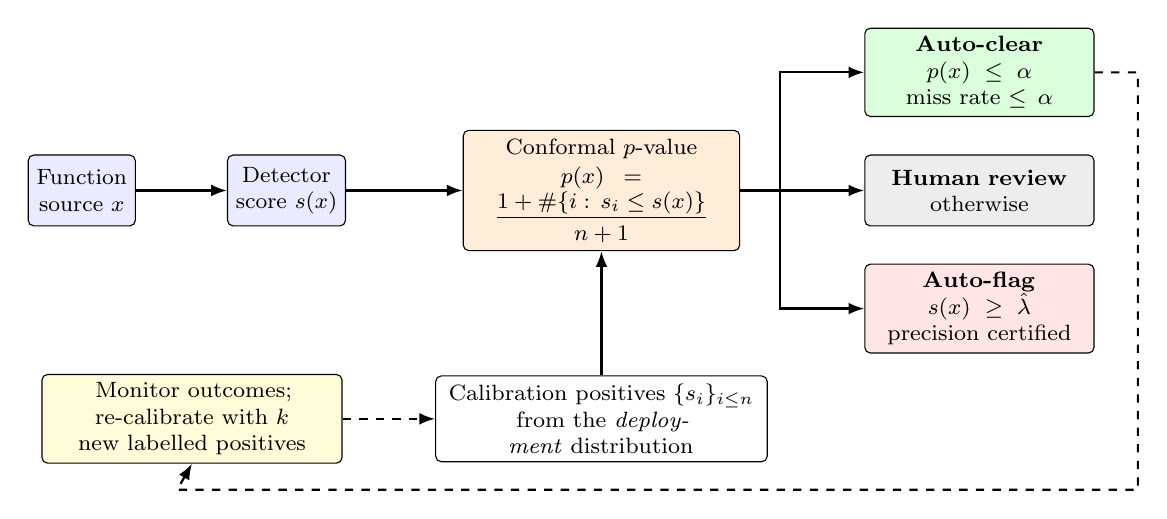
\begin{tikzpicture}[font=\footnotesize,
  box/.style={draw, rounded corners=2pt, align=center, inner sep=3pt, fill=#1, minimum height=9mm},
  box/.default=white, arr/.style={-{Latex[length=2mm]}, thick}]
  \node[box=blue!8] (fn) at (0,0) {Function\\source $x$};
  \node[box=blue!8] (det) at (2.6,0) {Detector\\score $s(x)$};
  \node[box=orange!15, text width=33mm] (p) at (6.6,0) {Conformal $p$-value\\[1pt]$p(x)=\dfrac{1+\#\{i:\,s_i\le s(x)\}}{n+1}$};
  \node[box=green!14, text width=27mm] (clear) at (11.4,1.5) {\textbf{Auto-clear}\\$p(x)\le\alpha$\\miss rate $\le\alpha$};
  \node[box=gray!14, text width=27mm] (rev) at (11.4,0) {\textbf{Human review}\\otherwise};
  \node[box=red!10, text width=27mm] (fl) at (11.4,-1.5) {\textbf{Auto-flag}\\$s(x)\ge\hat\lambda$\\precision certified};
  \node[box=white, text width=40mm] (cal) at (6.6,-2.9) {Calibration positives $\{s_i\}_{i\le n}$\\from the \emph{deployment} distribution};
  \node[box=yellow!15, text width=36mm] (mon) at (1.4,-2.9) {Monitor outcomes;\\re-calibrate with $k$ new labelled positives};
  \draw[arr] (fn)--(det); \draw[arr] (det)--(p);
  \draw[arr] (p.east) -- ++(0.5,0) |- (clear.west);
  \draw[arr] (p.east) -- (rev.west);
  \draw[arr] (p.east) -- ++(0.5,0) |- (fl.west);
  \draw[arr] (cal)--(p);
  \draw[arr, dashed] (mon)--(cal);
  \draw[arr, dashed] (clear.east) -- ++(0.55,0) -- ++(0,-5.3) -- ++(-12.2,0) -- (mon.south);
\end{tikzpicture}
}
\caption{Risk-controlled triage. Calibration positives from the deployment distribution fix the clearance threshold; a function is auto-cleared when its conformal $p$-value is at most the miss budget $\alpha$, auto-flagged when a certified precision threshold is met, and reviewed otherwise. Outcomes feed back into re-calibration.}\label{fig:framework}
\end{figure}

\paragraph{Findings in brief} We test the construction on 487\,412 deduplicated C/C++ functions from two public corpora (DiverseVul and Big-Vul), in seven evaluation scenarios (random, project-disjoint, temporal, cross-dataset), with three seeds and four detectors, together with a rule-based analyser. The guarantee is exact on exchangeable data and fails under every kind of shift we examine, by a factor of 2.7 on average; the standard remedy of covariate-shift weighting does not repair it; and a small number of labelled target positives (about 100) does. What can then be automated is about half of what a random-split evaluation suggests.

\paragraph{Contributions}
\begin{enumerate}[itemsep=1pt]
\item \textbf{Formulation and theory.} A risk-control formulation of vulnerability triage with operational quantities (miss rate, safe automation rate, review effort) and the following results: validity and calibration-set variability of conformal clearance (Prop.~\ref{prop:valid}, Cor.~\ref{cor:beta}), a high-probability variant (Prop.~\ref{prop:pac}), a bound on the miss-rate excess under shift in terms of the KS distance (Prop.~\ref{prop:shift}), group-conditional validity (Prop.~\ref{prop:mondrian}), the identity $\mathrm{AUROC}=\int\mathrm{TNR}(\alpha)d\alpha$ that explains why AUROC is a poor proxy for operational value (Lemma~\ref{lem:auc}), and an economically optimal miss budget (Prop.~\ref{prop:cost}).
\item \textbf{A shift-aware empirical test of the guarantee} on seven scenarios, including evidence that source-calibrated clearance misses $2.7\times$ the nominal share under shift, that all 336 observations satisfy the proposed bound, that covariate-shift weighting is insufficient, and how many labelled target positives are needed to recover validity.
\item \textbf{A data-quality and leakage audit} of DiverseVul and Big-Vul (24.6\% exact duplicates in Big-Vul; 42.7\% of Big-Vul inside DiverseVul) and its quantified effect on cross-dataset evaluation.
\item \textbf{Accountability analyses}: uneven miss rates across function sizes and CWEs and their repair by Mondrian calibration; decision flips under semantics-preserving rewrites; a TreeSHAP fidelity/consistency study that links the model's reliance on function size to the unevenness.
\item \textbf{Operational evidence}: comparison with a rule-based analyser and a cost analysis that shows when delegation pays off.
\item \textbf{An open, reproducible artifact} that regenerates every number in this paper from cached scores.
\end{enumerate}

\paragraph{Scope} Because the study had to be completed on CPU-only infrastructure, the detectors are TF-IDF/gradient-boosting models rather than fine-tuned code language models. The triage layer is detector-agnostic and the theoretical conclusions do not depend on the scorer, but the numerical levels (for example the achievable SAR) will differ for stronger models; Section~\ref{sec:threats} discusses this.

\paragraph{Structure} Section~\ref{sec:related} places the work in the literature, Section~\ref{sec:method} develops the theory, Section~\ref{sec:design} describes the study, Section~\ref{sec:results} answers the five research questions, and Sections~\ref{sec:discussion}--\ref{sec:conclusion} discuss implications, threats and conclusions.

\section{Background and related work}\label{sec:related}

\paragraph{Learning-based vulnerability detection and its evaluation}
Function-level detectors based on graph networks~\cite{zhou2019devign}, token models and pre-trained code language models are commonly reported with high accuracy on random splits of public corpora. Chakraborty et al.~\cite{chakraborty2021deep} showed that performance drops sharply on realistic data, and recent studies with PrimeVul~\cite{ding2024primevul} reach similar conclusions for code language models under de-duplicated, time-aware evaluation. The data underneath is itself a threat: label noise and duplication in vulnerability corpora are documented~\cite{croft2023data}, and code duplication inflates the results of machine-learning models of code~\cite{allamanis2019adverse}. The same concern about space--time bias is well established in malware detection~\cite{pendlebury2019tesseract}. Our audit (Section~\ref{sec:design}) and the leakage experiment (Section~\ref{sec:rq1}) quantify these issues for the two corpora we use and carry the analysis one step further, from how \emph{accurate} a detector is to what a team can \emph{safely delegate} to it.

\paragraph{Calibration, selective prediction and uncertainty}
Neural networks are often miscalibrated~\cite{guo2017calibration} and post-hoc scaling and isotonic regression are standard remedies. Selective classification lets a model abstain on uncertain inputs and trades coverage for risk~\cite{geifman2017selective}. Uncertainty estimation has begun to appear in vulnerability detection, for example Bayesian recurrent detectors and toolkits that quantify the uncertainty of code language models. These approaches provide \emph{scores}, not statistical guarantees on the error of the delegated decisions, and calibration alone does not give a guarantee on a specified class-conditional error such as the share of missed vulnerabilities.

\paragraph{Conformal prediction and risk control}
Conformal prediction~\cite{vovk2005algorithmic,shafer2008tutorial,angelopoulos2021gentle} converts any scorer into a procedure with finite-sample, distribution-free coverage under exchangeability; conformal risk control~\cite{angelopoulos2023conformal} and Learn-then-Test~\cite{angelopoulos2021ltt} generalise it to controlling expected loss and to high-probability statements about arbitrary risks; weighted conformal prediction~\cite{tibshirani2019conformal} extends validity to covariate shift with a known likelihood ratio. Class-conditional miss-rate control of this kind is used for safety warning systems in robotics~\cite{luo2022sample}. To the best of our knowledge, and based on our literature search, the application of such guarantees to \emph{automated vulnerability triage}, together with an empirical analysis of how the guarantee behaves under the project, temporal and cross-dataset shifts that characterise software evolution, has not been studied before. Our contribution is not a new conformal theory, but (i) its specialisation to the clearance decision of a vulnerability detector, with a diagnostic bound on the effect of shift (Proposition~\ref{prop:shift}), the high-probability variant, and an economic rule for choosing the budget; and (ii) a large empirical test of when these guarantees hold in practice.

\paragraph{Static analysis and alert fatigue}
Rule-based analysers produce many alerts that developers ignore~\cite{johnson2013why}. We include Flawfinder as a representative lightweight analyser and compare it with the learned triage layer on identical functions.

\paragraph{Robustness and explanation of code models}
Models of code are sensitive to semantics-preserving transformations such as identifier renaming~\cite{rabin2021generalizability,yefet2020adversarial}. For trustworthy automation what matters is whether the \emph{delegated decision} changes, so we measure decision flips of the triage layer rather than only score changes. For explanation we use TreeSHAP~\cite{lundberg2017shap,lundberg2020treeshap} on an interpretable metric-based model, evaluate fidelity by deletion, and test consistency of the explanations across seeds and across datasets.

\section{Risk-controlled triage: formulation and guarantees}\label{sec:method}

This section formalises the triage layer and states the guarantees that the empirical study (Section~\ref{sec:design}) tests.
All proofs are short and are given in full so that the assumptions under which each guarantee holds, and therefore the conditions under which it fails, are explicit.

\subsection{Setting and operational quantities}
Let $X$ be a function (source text) and $Y\in\{0,1\}$ indicate that it is vulnerable, with prevalence $\pi=\Pr(Y=1)$.
A trained detector yields a real-valued \emph{score} $S=s(X)$, where larger values indicate higher vulnerability likelihood; $s$ may be any monotone proxy of a probability (a logit, a margin, or a calibrated probability).
For a distribution $P$ over $(X,Y)$ and a threshold $\tau$ we define

\begin{align}
  M_P(\tau) &= \Pr\nolimits_P\!\left(S\le\tau \mid Y=1\right),\label{eq:miss}\\
  \mathrm{TNR}_P(\tau) &= \Pr\nolimits_P\!\left(S\le\tau \mid Y=0\right),\\
  \mathrm{SAR}_P(\tau) &= \Pr\nolimits_P\!\left(S\le\tau\right).\label{eq:sar}
\end{align}
Here $M$ is the \emph{miss rate} (the share of vulnerable functions that are auto-cleared), $\mathrm{TNR}$ the share of benign functions that are auto-cleared, and $\mathrm{SAR}$ the \emph{safe automation rate}, the share of all functions that are auto-cleared.

A triage policy with clearance threshold $\tau_c$ and flag threshold $\tau_f\ge\tau_c$ assigns every function to one of three outcomes: \emph{clear} if $S\le\tau_c$, \emph{flag} if $S\ge\tau_f$, and \emph{review} otherwise.
Only the clear decision removes a function from human attention without evidence, so it is the decision that must carry a safety guarantee; flagging consumes (or, with certification, saves) reviewer time but does not hide vulnerabilities.

\begin{lemma}[Decomposition of automation]\label{lem:sar}
$\mathrm{SAR}(\tau)=(1-\pi)\,\mathrm{TNR}(\tau)+\pi\,M(\tau)$.
When nothing is auto-flagged, the expected number of functions a team must review per 1\,000 is $\mathrm{ERE}(\tau)=1000\,\bigl(1-\mathrm{SAR}(\tau)\bigr)$.
\end{lemma}
\begin{proof}
Condition on $Y$ in the law of total probability: $\Pr(S\le\tau)=\Pr(S\le\tau\mid Y{=}0)(1-\pi)+\Pr(S\le\tau\mid Y{=}1)\pi$.
\end{proof}

Because $\pi\approx 5\%$ in realistic data, Lemma~\ref{lem:sar} shows that automation is driven almost entirely by $\mathrm{TNR}$ at the chosen miss budget $M(\tau)=\alpha$.
Write $\mathrm{TNR}(\alpha)$ for the true-negative rate at the threshold whose miss rate is $\alpha$ (the ROC curve reflected in $\alpha=1-\mathrm{TPR}$).

\begin{lemma}[AUROC is the average clearance potential]\label{lem:auc}
If the score distributions are continuous, $\mathrm{AUROC}=\int_0^1 \mathrm{TNR}(\alpha)\,d\alpha$.
\end{lemma}
\begin{proof}
Let $F_1,F_0$ be the score CDFs of vulnerable and benign functions, so $\mathrm{TNR}(\alpha)=F_0(F_1^{-1}(\alpha))$.
With $U\sim\mathrm{Unif}(0,1)$, $F_1^{-1}(U)$ has the law of a vulnerable score $S_1$; hence $\int_0^1F_0(F_1^{-1}(\alpha))d\alpha=\mathbb E[F_0(S_1)]=\Pr(S_0\le S_1)=\mathrm{AUROC}$ for an independent benign score $S_0$.
\end{proof}

Lemma~\ref{lem:auc} explains why AUROC is a poor proxy for \emph{operational} value: a safety-relevant budget such as $\alpha=0.05$ uses only the left tail of the integral, and two detectors with equal AUROC can differ widely in $\mathrm{TNR}(0.05)$.
Section~\ref{sec:rq1} quantifies this.

\subsection{Conformal clearance with a finite-sample miss-rate guarantee}
Let $s_1,\dots,s_n$ be the scores of $n$ \emph{vulnerable} functions in a held-out calibration set, and define for a new function $x$ with score $s$ the conformal $p$-value
\begin{equation}
  p(x)=\frac{1+\#\{i\le n:\ s_i\le s\}}{n+1}.\label{eq:pval}
\end{equation}
The policy \emph{clears $x$ iff $p(x)\le\alpha$}. Equivalently, with $s_{(1)}\le\dots\le s_{(n)}$ the order statistics and $k=\lfloor\alpha(n+1)\rfloor$, it clears iff $s<s_{(k)}$ (and clears nothing if $k=0$).

\begin{proposition}[Finite-sample validity]\label{prop:valid}
If the score $S_{n+1}$ of a vulnerable test function is exchangeable with $s_1,\dots,s_n$, then $\Pr\bigl(p(X_{n+1})\le\alpha\bigr)\le\alpha$ for every $\alpha\in(0,1)$; that is, the expected miss rate of the clearance rule is at most $\alpha$.
If scores are almost surely distinct the probability is exactly $\lfloor\alpha(n+1)\rfloor/(n+1)\ge\alpha-\tfrac1{n+1}$.
\end{proposition}
\begin{proof}
Let $R=1+\#\{i\le n: s_i\le S_{n+1}\}$ so that $p=R/(n+1)$. $R$ is at least the rank of $S_{n+1}$ among the $n{+}1$ scores under uniformly random tie-breaking, and that rank is uniform on $\{1,\dots,n{+}1\}$ by exchangeability. Hence $\Pr(R\le k)\le k/(n+1)$, and $p\le\alpha\iff R\le\lfloor\alpha(n+1)\rfloor$. With distinct scores $R$ is the rank itself, giving equality.
\end{proof}

\begin{corollary}[Calibration-set variability and minimum sample size]\label{cor:beta}
For continuous scores, the \emph{conditional} miss rate given the calibration set, $M(\hat\tau)$, follows $\mathrm{Beta}(k,\,n+1-k)$ with $k=\lfloor\alpha(n+1)\rfloor$.
Its mean is $k/(n+1)\le\alpha$ and its variance is $\approx\alpha(1-\alpha)/(n+2)$. A non-trivial rule requires $n\ge\lceil1/\alpha\rceil-1$ calibration positives.
\end{corollary}
\begin{proof}
The rule clears $s<s_{(k)}$, so $M(\hat\tau)=F_1(s_{(k)}^-)$, the $k$-th order statistic of $n$ i.i.d.\ Uniform$(0,1)$ variables after the probability integral transform, which is $\mathrm{Beta}(k,n{+}1{-}k)$.
\end{proof}

Proposition~\ref{prop:valid} is a \emph{marginal} (expected) guarantee: roughly half of independent calibration draws will produce a realised miss rate slightly above $\alpha$ (Corollary~\ref{cor:beta}).
A practitioner who needs a high-probability statement can use the following variant.

\begin{proposition}[PAC clearance]\label{prop:pac}
Fix $\delta\in(0,1)$ and let $j^\star=\max\{j:\ F^{-1}_{\mathrm{Beta}(j,\,n+1-j)}(1-\delta)\le\alpha\}$. Clearing iff $s<s_{(j^\star)}$ satisfies $\Pr_{\text{calibration}}\bigl(M(\hat\tau)>\alpha\bigr)\le\delta$ for continuous, exchangeable scores (and clears nothing if no such $j$ exists).
\end{proposition}
\begin{proof}
By Corollary~\ref{cor:beta}, $M(\hat\tau)\sim\mathrm{Beta}(j^\star,n{+}1{-}j^\star)$, and $j^\star$ is chosen so that its $(1-\delta)$ quantile does not exceed $\alpha$.
\end{proof}

\subsection{What distribution shift does to the guarantee}
Exchangeability is the only assumption in Proposition~\ref{prop:valid}, and it is exactly what project-level, temporal and cross-dataset evaluation violate.
Let $F_c$ and $F_t$ be the CDFs of the scores of vulnerable functions under the calibration and test distributions, and $D=\sup_s|F_c(s)-F_t(s)|$ their Kolmogorov--Smirnov distance.

\begin{proposition}[Shift bound]\label{prop:shift}
For a threshold $\hat\tau$ calibrated at level $\alpha$ under $P_c$ with $n$ positives,
\[
\mathbb E\bigl[M_{P_t}(\hat\tau)\bigr]\ \le\ \alpha + D .
\]
The bound is attained when $F_t$ lies uniformly $D$ above $F_c$ at the clearance threshold.
\end{proposition}
\begin{proof}
Pointwise $F_t(\tau)\le F_c(\tau)+D$ for every $\tau$, hence $M_{P_t}(\hat\tau)=F_t(\hat\tau^-)\le F_c(\hat\tau^-)+D$. Taking expectations over the calibration draw and applying Proposition~\ref{prop:valid} to the first term gives the claim.
\end{proof}

Proposition~\ref{prop:shift} is not a repair but a \emph{diagnostic}: the excess miss rate over the nominal budget cannot exceed the KS distance between the positive-class scores before and after the shift. Figure~\ref{fig:ks} tests this bound on every shifted scenario.
Two remedies are studied.

\paragraph{Covariate-shift weighting}
If $\Pr_t(Y|x)=\Pr_c(Y|x)$ and $w(x)=dP_t(x)/dP_c(x)$ is known, the likelihood ratio on the positive class is $w(x)\,\pi_c/\pi_t$; the constant cancels after normalisation, so the weighted $p$-value of Tibshirani et al.~\cite{tibshirani2019conformal},
\begin{equation}
  p_w(x)=\frac{\sum_{i=1}^n w(x_i)\,\mathbb 1[s_i\le s]+w(x)}{\sum_{i=1}^n w(x_i)+w(x)},
\end{equation}
restores validity when computed on the calibration \emph{positives}. We estimate $w$ with a cross-fitted logistic domain classifier on TF-IDF features. The guarantee is only as good as the density-ratio estimate and the covariate-shift assumption, both of which are doubtful for code; we therefore treat it as an empirical question (RQ3).

\paragraph{Recalibration on a small labelled target sample}
If $k$ labelled vulnerable functions from the \emph{target} distribution (the new project, or the most recent release window) are available, calibrating on them restores exchangeability by construction, and Proposition~\ref{prop:valid} applies verbatim with $n=k$. The price is variance: by Corollary~\ref{cor:beta}, the realised miss rate has standard deviation $\approx\sqrt{\alpha(1-\alpha)/k}$, and the PAC variant (Proposition~\ref{prop:pac}) trades part of the clearance rate for a bounded violation probability.

\subsection{Online risk control under drift}\label{sec:online}
Recalibration on a labelled target sample (Section above) is a one-off remedy. In deployment the distribution keeps moving (new releases, new projects) and labels arrive over time: a vulnerable function that was cleared may be discovered later (an incident, a disclosure, an audit of the cleared pool). We therefore also consider a stream of functions processed in batches $b=1,2,\dots$ with \emph{delayed feedback}: the labels of batch $b$ become known after the batch has been decided.

Adaptive conformal inference (ACI)~\cite{gibbs2021adaptive} turns the miss budget into a control variable. Let $\alpha_1=\alpha$ and, for batch $b$, clear iff $s<s^{\mathrm{ref}}_{(k_b)}$ with $k_b=\lfloor\alpha_b(n+1)\rfloor$ computed on a reference set of $n$ vulnerable scores (the source calibration positives, or the most recent $W$ observed vulnerable functions); the rule clears nothing if $\alpha_b\le0$ and everything if $\alpha_b\ge1$. After the batch, for each vulnerable function $i$ of the batch in turn, with $e_i=1$ if it was cleared and $0$ otherwise,
\begin{equation}
  \alpha\leftarrow\alpha+\gamma\,(\alpha_{\mathrm{target}}-e_i).\label{eq:aci}
\end{equation}
\begin{proposition}[Online miss-rate control with delayed feedback]\label{prop:online}
Let $b_{\max}$ be the largest number of vulnerable functions in a batch and $N$ the total number of vulnerable functions in the stream. For \emph{any} sequence of scores and labels (no exchangeability, no assumption on the shift),
\[
\Bigl|\frac1N\sum_{i=1}^N e_i-\alpha\Bigr|\ <\ \frac{1+\gamma\,b_{\max}}{\gamma\,N}.
\]
\end{proposition}
\begin{proof}
Summing~\eqref{eq:aci} over all vulnerable functions gives $\sum_i(\alpha-e_i)=(\alpha_{\mathrm{end}}-\alpha_1)/\gamma$, so it suffices to bound the final level. Consider the level $a$ at the start of a batch. If $a\le0$ nothing is cleared, every $e_i=0$ and the level can only increase within the batch. If $a>0$ it decreases by at most $\gamma(1-\alpha)$ per vulnerable function, hence stays above $-\gamma b_{\max}(1-\alpha)$; by induction over batches the level never falls below this value. Symmetrically, if $a\ge1$ everything is cleared, every $e_i=1$ and the level can only decrease, while if $a<1$ it increases by at most $\gamma\alpha$ per vulnerable function, so the level stays below $1+\gamma b_{\max}\alpha$. Hence $-\gamma b_{\max}(1-\alpha)-\alpha<\alpha_{\mathrm{end}}-\alpha_1<1+\gamma b_{\max}\alpha-\alpha$, and $\lvert\alpha_{\mathrm{end}}-\alpha_1\rvert<1+\gamma b_{\max}$.
\end{proof}
Proposition~\ref{prop:online} is a guarantee on the \emph{long-run average} miss rate of the whole stream, deterministic in the data; it says nothing about the miss rate in a given window, which is why we also report the worst window. Its price is automation: if the scorer degrades, the level $\alpha_b$ falls and fewer functions are cleared. It requires feedback on every vulnerable function, including the cleared ones; with feedback on a random fraction $q$ of the cleared functions, $e_i/q$ is an unbiased replacement (not evaluated here). The proof does not depend on the reference set, so the bound also holds when the reference is a sliding window of observed vulnerable scores (``ACI+window'').

\subsection{Group-conditional validity (Mondrian calibration)}
The marginal guarantee averages over all vulnerable functions and can hide very uneven risk across inputs that are observable at inference time.
Partition the input space by a function $b(x)$ (we use function-length terciles).
\begin{proposition}[Mondrian validity]\label{prop:mondrian}
If clearance in group $g$ uses $p$-values computed only from calibration positives with $b=g$, then for every group $g$ with exchangeable calibration and test positives, $\Pr\bigl(p_g(X)\le\alpha\mid Y{=}1, b(X){=}g\bigr)\le\alpha$.
\end{proposition}
\begin{proof}
Condition on $b(X_{n+1})=g$ and on the set of calibration indices in group $g$; scores within the group remain exchangeable, and Proposition~\ref{prop:valid} applies with $n$ replaced by the group's calibration size.
\end{proof}

\subsection{Certified auto-flagging}
Flagging with a guarantee on precision is the dual problem, and harder because it is conditioned on the predicted class.
We use the Learn-then-Test fixed-sequence procedure~\cite{angelopoulos2021ltt}: half of the calibration set fixes a descending grid of thresholds $\lambda_1>\lambda_2>\cdots$; on the other half we test, in order, $H_j:\ \Pr(Y{=}1\mid S\ge\lambda_j)<\beta$ with a one-sided Clopper--Pearson bound at level $\delta$, and stop at the first non-rejection. The last rejected threshold $\hat\lambda$ then satisfies $\Pr\bigl(\Pr(Y{=}1\mid S\ge\hat\lambda)<\beta\bigr)\le\delta$.
Because precision of vulnerability detectors is low (Section~\ref{sec:rq3}), we expect few or no certifiable flags at practically useful $\beta$; this is itself a finding about what can safely be automated.

\subsection{Choosing the miss budget economically}
Let one human review cost $1$ and one missed vulnerability cost $c_m$ (in review units). The expected cost per function when clearing at miss budget $\alpha$ is
\begin{equation}
  C(\alpha)=\bigl(1-\mathrm{SAR}(\alpha)\bigr)+c_m\,\pi\,\alpha ,\label{eq:cost}
\end{equation}
to be compared with $C=1$ for ``review everything'' and $C=c_m\pi$ for ``review nothing''.
\begin{proposition}[Cost-optimal budget]\label{prop:cost}
For differentiable $\mathrm{TNR}(\cdot)$, an interior minimiser of~\eqref{eq:cost} satisfies
\[
 \mathrm{TNR}'(\alpha^\star)\;=\;\frac{\pi\,(c_m-1)}{1-\pi}.
\]
\end{proposition}
\begin{proof}
By Lemma~\ref{lem:sar}, $\mathrm{SAR}(\alpha)=(1-\pi)\mathrm{TNR}(\alpha)+\pi\alpha$, so $C'(\alpha)=-(1-\pi)\mathrm{TNR}'(\alpha)-\pi+c_m\pi$; set it to zero.
\end{proof}
Since $\mathrm{TNR}'(\alpha)$ is decreasing for concave ROC curves, larger $c_m$ pushes $\alpha^\star$ down; if $\mathrm{TNR}'(\alpha)<\pi(c_m-1)/(1-\pi)$ already at $\alpha\to0$ the optimum is to review everything. Section~\ref{sec:rq5} evaluates $\alpha^\star$ chosen on calibration data against realised cost on the test data.

\subsection{Algorithm}
Algorithm~\ref{alg:triage} summarises calibration and deployment. The calibration step costs one sort of the positive calibration scores; inference adds one binary search per function.

\begin{algorithm}[t]
\caption{Risk-controlled triage (calibration and deployment)}\label{alg:triage}
\begin{algorithmic}[1]
\Require trained scorer $s(\cdot)$; labelled calibration set $\mathcal D_{\mathrm{cal}}$ \emph{from the deployment distribution}; miss budget $\alpha$; optional PAC level $\delta$; optional group map $b(\cdot)$
\State $\mathcal S^+\gets\{s(x_i): (x_i,y_i)\in\mathcal D_{\mathrm{cal}},\ y_i=1\}$, sorted; $n\gets|\mathcal S^+|$ (per group if Mondrian)
\State $k\gets\lfloor\alpha(n+1)\rfloor$ \textbf{or} $k\gets j^\star(n,\alpha,\delta)$ for the PAC variant; \textbf{if} $k=0$ \textbf{then} clear nothing
\State $\hat\tau\gets s_{(k)}$ (clear iff $s(x)<\hat\tau$)
\For{each new function $x$}
  \State \textbf{if} $s(x)<\hat\tau$ \textbf{then} auto-clear \textbf{else} send to review (or auto-flag if $s(x)\ge\hat\lambda$)
\EndFor
\State Monitor: on every batch of newly labelled outcomes, update the level with Eq.~\eqref{eq:aci} (ACI) or recalibrate on the most recent observed vulnerable functions
\end{algorithmic}
\end{algorithm}

\section{Empirical study design}\label{sec:design}

\subsection{Research questions}
\begin{description}[leftmargin=2.2em,style=nextline,itemsep=2pt]
\item[RQ1 (Reliability of detection).] How much does the detection quality of learning-based detectors drop when the evaluation moves from a random split to project-disjoint, temporal and cross-dataset conditions, and is AUROC a faithful predictor of operational value?
\item[RQ2 (Calibration).] How well-calibrated are the probabilities of these detectors, and how much do post-hoc recalibration methods help under shift?
\item[RQ3 (Guarantees under shift).] Does the conformal clearance rule keep its miss-rate budget when calibrated on source data, and which remedies (covariate-shift weighting, labelled target recalibration, the PAC variant) restore it? How many labelled target positives are needed?
\item[RQ4 (Accountability).] Is the guarantee distributed evenly across function sizes and vulnerability classes (CWEs), and does Mondrian calibration repair imbalances? How consistent are the triage decisions and the explanations under semantics-preserving rewrites and across datasets?
\item[RQ5 (Operational value).] How much reviewer effort does risk-controlled triage save at a valid miss budget, how does it compare with a rule-based static analyser, and what does it imply under an explicit cost model?
\item[RQ6 (Pre-trained code model).] Do the conclusions hold for a scorer built on a pre-trained code model (CodeBERT), and do such models exploit dataset artifacts that lexical models cannot see?
\end{description}

\subsection{Datasets and data-quality audit}
We use two public C/C++ function-level vulnerability datasets that differ in provenance.
\textbf{DiverseVul}~\cite{chen2023diversevul} contains functions collected from security-issue websites and the commits that fix them; each record carries the project, the fixing commit and (where available) the CWE.
\textbf{Big-Vul}~\cite{fan2020bigvul} links CVE records to fixing commits; we use the pre-fix function body as the vulnerable sample, the unchanged functions from the same commits as benign samples, and take the publication year from the CVE identifier as a temporal key.
Both were obtained from the Hugging Face hub (\texttt{claudios/DiverseVul}, \texttt{bstee615/bigvul}).
We deliberately did not use the Juliet test suite, whose synthetic flaws make random-split results saturate, nor PrimeVul, which was not retrievable in our environment.

\paragraph{Pre-processing and audit}
For each function we strip comments, collapse whitespace and hash the result. Within a dataset we remove exact duplicates, and we drop every hash that occurs with conflicting labels. Across datasets we compute the overlap of normalised hashes.
Table~\ref{tab:data} reports the audit; the consequences for evaluation are discussed in Section~\ref{sec:rq1}.

\begin{table}[t]
\centering\footnotesize
\caption{Dataset audit after normalisation (comment/whitespace stripping). 69,268 normalised functions occur in both datasets: 42.7\% of clean Big-Vul and 21.3\% of clean DiverseVul.}\label{tab:data}
\resizebox{\linewidth}{!}{\begin{tabular}{lrrrrrr}
\toprule
Dataset & Raw & Exact duplicates & Label-conflict & Clean & Vulnerable & Projects \\
\midrule
DiverseVul & 328,907 & 3,025 (0.9\%) & 1,497 & 325,138 & 17,689 (5.4\%) & 800 \\
Big-Vul & 216,568 & 53,373 (24.6\%) & 2,333 & 162,274 & 8,055 (5.0\%) & 309 \\
\bottomrule
\end{tabular}}
\end{table}


\subsection{Evaluation scenarios}
Table~\ref{tab:scen} defines seven scenarios. In every scenario the detector is trained on the \emph{train} part; the \emph{ID calibration} part is a random hold-out of the training distribution (what a practitioner would naturally use); the \emph{test} part is where all reported numbers are measured; and, for the shifted scenarios, a labelled \emph{target pool} drawn from the deployment distribution is available for the recalibration experiments but disjoint from the test part.
\begin{itemize}[itemsep=1pt]
\item \textbf{Random} (DV-R, BV-R): 70/15/15 split of deduplicated functions; calibration and test are exchangeable.
\item \textbf{Project} (DV-P, BV-P): 70\% of projects are used for training and calibration; the remaining projects form the test set (a new codebase is deployed). A random 25\% of the held-out projects' functions is the target pool.
\item \textbf{Temporal} (BV-T): train and ID calibration on CVEs published up to 2015, target pool = 2016, test = 2017--2019 (a model deployed on newer vulnerabilities).
\item \textbf{Cross-dataset} (DV$\to$BV, BV$\to$DV): train on 85\% of one dataset, calibrate on the remaining 15\%, test on the other dataset after \emph{removing every test function whose normalised hash occurs in the training data}; a random 25\% of the remaining target data is the pool. Removed (leaked) functions are evaluated separately to measure how much leakage would have inflated the result.
\end{itemize}
Each scenario is repeated with three seeds (different partitions and model initialisations).

\begin{table}[t]
\centering\footnotesize
\caption{Evaluation scenarios (seed 0 sizes; training keeps all vulnerable and at most 150\,000 benign functions).}\label{tab:scen}
\resizebox{\linewidth}{!}{\begin{tabular}{llrrrrr}
\toprule
Scenario & Shift & Train & ID cal. & Target pool & Test & Test pos. \\
\midrule
DV random & random 70/15/15 & 162,475 & 48,879 & -- & 48,553 & 2,637 \\
BV random & random 70/15/15 & 113,482 & 24,489 & -- & 24,303 & 1,254 \\
DV project & held-out projects (30\%) & 159,829 & 30,432 & 31,053 & 91,423 & 4,522 \\
BV project & held-out projects (30\%) & 124,551 & 22,227 & 3,826 & 11,670 & 699 \\
BV temporal & train $\le$2015; test 2017--19 & 60,101 & 10,850 & 27,022 & 52,669 & 2,288 \\
DV$\to$BV & train DV, test BV (leak-free) & 165,052 & 48,553 & 25,869 & 77,380 & 4,240 \\
BV$\to$DV & train BV, test DV (leak-free) & 137,971 & 24,303 & 66,735 & 199,348 & 11,207 \\
\bottomrule
\end{tabular}}
\end{table}


\subsection{Detectors}
Because the experiments must be fully reproducible on commodity CPUs and over 20 scenario--seed pairs, we use four lightweight, widely used detectors on the full corpora, complemented by a frozen-CodeBERT experiment on a subsample (Section~\ref{sec:design_cb}); the absence of fine-tuned code models is a limitation discussed in Section~\ref{sec:threats}, and the triage layer is detector-agnostic.
\begin{itemize}[itemsep=1pt]
\item \textbf{TF-IDF LR} and \textbf{TF-IDF SVM}: unigram+bigram code tokens hashed to $2^{19}$ features, sublinear TF-IDF, logistic regression ($C{=}20$) or linear SVM ($C{=}0.3$).
\item \textbf{LightGBM}~\cite{ke2017lightgbm}: gradient-boosted trees on 71 engineered code metrics (size, nesting depth, cyclomatic proxy, pointer/cast/bit-operation counts, counts of 32 security-relevant API calls) plus the 20\,000 most frequent hashed tokens; early stopping on 10\% of the training data.
\item \textbf{LR+LGBM}: sum of standardised LR margin and LightGBM logit.
\end{itemize}
Training sets keep all vulnerable functions and at most 150\,000 benign ones; this does not affect the triage layer, which depends on score ranks only.
The rule-based baseline is \textbf{Flawfinder} 2.0.20, with the highest risk level among a function's hits (then the number of hits) as score.

\subsection{Pre-trained code model experiment (RQ6)}\label{sec:design_cb}
To test whether the findings depend on the lightweight detectors, we add scorers built on CodeBERT~\cite{feng2020codebert} (\texttt{microsoft/codebert-base}). Because the study ran without a GPU, the encoder is \emph{frozen}: we embed the first 256 tokens of each function and use the concatenation of the [CLS] vector and the mean-pooled last layer (1\,536 dimensions) as features of a standardised logistic regression ($C{=}0.05$) and of a LightGBM (embedding plus the 71 code metrics); their standardised sum is the ``CodeBERT ensemble''. Embedding the full corpora (487\,000 functions) is infeasible on CPU, so we use a stratified subsample of each corpus with all scenarios, splits and seeds unchanged: 5\,000 vulnerable and 10\,000 benign functions per dataset (30\,000 in total; the benign functions are a uniform sample, so positive-class quantities such as the miss rate are unaffected, while AUPRC and SAR are weighted back to the true prevalence). All scorers in this experiment, including the TF-IDF models, are retrained on the subsample so that comparisons are matched.
Two input variants are evaluated: \emph{raw text}, and \emph{normalised text} (comments removed, whitespace collapsed), the same normalisation used in the main study. A \emph{formatting-only} LightGBM on 15 formatting statistics of the raw text (indentation, trailing whitespace, comment markers, line lengths) serves as a shortcut probe. For cross-dataset scenarios this experiment is stricter than the main study: any target function that occurs anywhere in the full source corpus is removed.

\subsection{Metrics}
\textbf{Detection:} AUROC, AUPRC, and F1, MCC, precision, recall at the F1-optimal threshold chosen on ID calibration data.
\textbf{Calibration:} expected calibration error with 15 equal-mass bins, $\mathrm{ECE}=\sum_b\frac{|B_b|}{n}\lvert\bar y_b-\bar p_b\rvert$, and the Brier score, for raw probabilities, Platt scaling and isotonic regression fitted on ID calibration data.
\textbf{Triage:} realised miss rate $M$ on test positives against the nominal $\alpha\in\{0.02,0.05,0.10,0.20\}$, the share of cleared functions (SAR, Eq.~\eqref{eq:sar}), the review effort ERE, and the violation frequency $\Pr(M>\alpha+0.02)$ across 200 random calibration draws of 300 positives (60 for the weighted variant); the $2$-point tolerance reflects the sampling error of the test-set miss rate.
For certified flagging we report the flagged share and the realised precision.
\textbf{Accountability:} miss rate per length tercile and per CWE.
\textbf{Robustness:} the share of triage decisions that change after identifier renaming, dead-code insertion, or both, and the miss rate on rewritten inputs.
\textbf{Explanation:} TreeSHAP~\cite{lundberg2020treeshap} deletion fidelity, rank stability and cross-dataset consistency of feature importances.
\textbf{Operational:} expected cost~\eqref{eq:cost} with the budget $\alpha^\star$ chosen on calibration data.

\subsection{Statistical protocol}
Results are reported as means over the three seeds with standard deviations. Detectors are compared with the Friedman test over the 21 scenario--seed blocks; paired comparisons with the best detector use the Wilcoxon signed-rank test and Cliff's $\delta$ as effect size.
Whether the realised miss rate exceeds its nominal level is tested with a one-sided Wilcoxon test on the per-block differences between realised and nominal miss rate. Relations between quantities (AUROC versus clearable share, KS distance versus excess miss rate) are measured with Spearman's $\rho$. All thresholds, hyper-parameters and splits are fixed before looking at test data; the 2-point tolerance and the budgets $\alpha$ are the only analysis choices and are reported in full.

\subsection{Implementation and availability}
All code (data preparation, feature extraction, models, triage layer, experiments, figure/table generation and this manuscript) is in the repository accompanying the paper, with a unit test that checks the clearance rule against its $p$-value definition and its finite-sample validity by simulation. Every number in the paper is produced by the scripts from cached detector scores.

\section{Results}\label{sec:results}

\subsection{RQ1: Detection quality collapses outside the random split, and AUROC hides what matters}\label{sec:rq1}

\paragraph{Data audit and leakage}
The audit (Table~\ref{tab:data}) shows that the corpora are less clean than their raw size suggests: 24.6\% of the Big-Vul rows (53\,373) are exact duplicates after normalisation, against 0.9\% for DiverseVul, and 69\,268 normalised functions occur in both corpora, i.e.\ 42.7\% of clean Big-Vul and 21.3\% of clean DiverseVul. In the cross-dataset scenarios, about 44\,000 functions of the evaluated target test part (more than a quarter of Big-Vul, and about 13\% of DiverseVul) also appear in the training data. Figure~\ref{fig:leak} and Table~\ref{tab:leak} show what this does to a naive cross-dataset evaluation: for the LR+LGBM scorer, AUPRC is $0.171$ on leak-free Big-Vul functions but $0.602$ on the leaked ones (3.5$\times$), and $0.144$ vs.\ $0.812$ (5.6$\times$) when training on Big-Vul and testing on DiverseVul. A cross-dataset result that does not remove shared functions would therefore report a performance that is between three and a half and almost six times better than what a new codebase would experience.

\begin{figure}[t]
\centering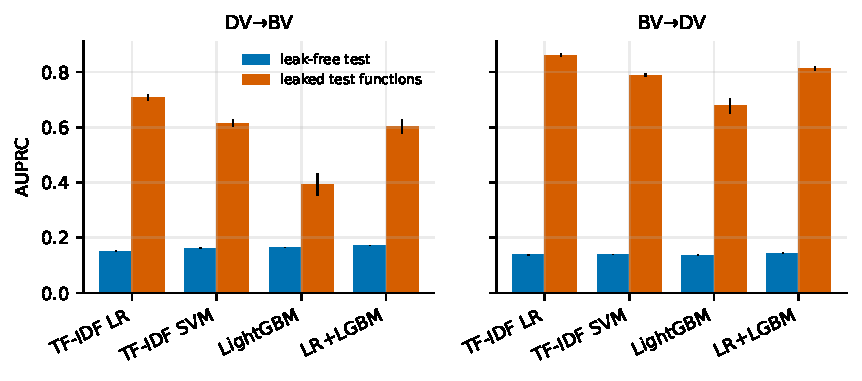
\includegraphics[width=.78\linewidth]{figs/fig_leak.pdf}
\caption{AUPRC on leak-free versus leaked cross-dataset test functions (mean $\pm$ s.d.\ over 3 seeds). The prevalence of vulnerable functions is about 5\%.}\label{fig:leak}
\end{figure}
\begin{table}[t]
\centering\footnotesize
\caption{Effect of train--test leakage in the cross-dataset setting: ``leaked'' test functions have a normalised hash that occurs in the training data.}\label{tab:leak}
\resizebox{\linewidth}{!}{\begin{tabular}{llrcccc}
\toprule
Scenario & Model & Leaked $n$ & AUPRC clean & AUPRC leaked & AUROC clean & AUROC leaked \\
\midrule
DV$\to$BV & TF-IDF LR & 44,180 & 0.151\,{\scriptsize$\pm$0.002} & 0.708\,{\scriptsize$\pm$0.010} & 0.679\,{\scriptsize$\pm$0.001} & 0.984\,{\scriptsize$\pm$0.002} \\
DV$\to$BV & LightGBM & 44,180 & 0.163\,{\scriptsize$\pm$0.000} & 0.392\,{\scriptsize$\pm$0.040} & 0.711\,{\scriptsize$\pm$0.003} & 0.877\,{\scriptsize$\pm$0.009} \\
DV$\to$BV & LR+LGBM & 44,180 & 0.171\,{\scriptsize$\pm$0.001} & 0.602\,{\scriptsize$\pm$0.026} & 0.710\,{\scriptsize$\pm$0.002} & 0.969\,{\scriptsize$\pm$0.002} \\
BV$\to$DV & TF-IDF LR & 44,120 & 0.137\,{\scriptsize$\pm$0.001} & 0.862\,{\scriptsize$\pm$0.005} & 0.711\,{\scriptsize$\pm$0.001} & 0.951\,{\scriptsize$\pm$0.003} \\
BV$\to$DV & LightGBM & 44,120 & 0.136\,{\scriptsize$\pm$0.002} & 0.679\,{\scriptsize$\pm$0.027} & 0.709\,{\scriptsize$\pm$0.006} & 0.909\,{\scriptsize$\pm$0.007} \\
BV$\to$DV & LR+LGBM & 44,120 & 0.144\,{\scriptsize$\pm$0.002} & 0.812\,{\scriptsize$\pm$0.007} & 0.721\,{\scriptsize$\pm$0.003} & 0.948\,{\scriptsize$\pm$0.002} \\
\bottomrule
\end{tabular}}
\end{table}


\paragraph{Performance under shift}
Table~\ref{tab:detect} and Figure~\ref{fig:detection} give the detection results. On random splits the LR+LGBM scorer reaches AUPRC $0.248$ (DiverseVul) and $0.407$ (Big-Vul); the percentages below are drops of this scorer, with AUROC $0.836$ and $0.869$. When whole projects are held out, AUPRC falls to $0.141$ (\,$-43\%$) and $0.151$ (\,$-63\%$); the temporal split on Big-Vul yields $0.113$ (\,$-72\%$), and the leak-free cross-dataset settings give $0.171$ and $0.144$. These values are only two to three times the prevalence ($\approx5\%$), and MCC drops to $0.12$--$0.17$ for the best model (Table~\ref{tab:detect}, panel C), against $0.29$ and $0.39$ on random splits. The ID-calibration AUPRC (what a practitioner would see on a hold-out of the training distribution) is $0.24$--$0.43$ in every scenario, so the optimism of in-distribution validation reaches $1.5$--$3.8\times$ for project, temporal and cross-dataset deployment ($0.264$ vs.\ $0.141$ for DiverseVul project, $0.425$ vs.\ $0.113$ for Big-Vul temporal).
The Friedman test over the 21 scenario--seed blocks rejects equal AUPRC for the four scorers ($\chi^2=21.9$, $p<10^{-4}$); the LR+LGBM scorer has the best mean rank ($1.48$), and beats TF-IDF LR ($p=0.011$, Cliff's $\delta=0.18$) and LightGBM ($p<10^{-5}$, $\delta=0.14$), while the difference to the SVM is borderline ($p=0.055$, $\delta=0.14$). Differences between scorers are small relative to the drop caused by the evaluation setting. We therefore use LR+LGBM as the scorer in the triage experiments unless stated otherwise.

\begin{figure}[t]
\centering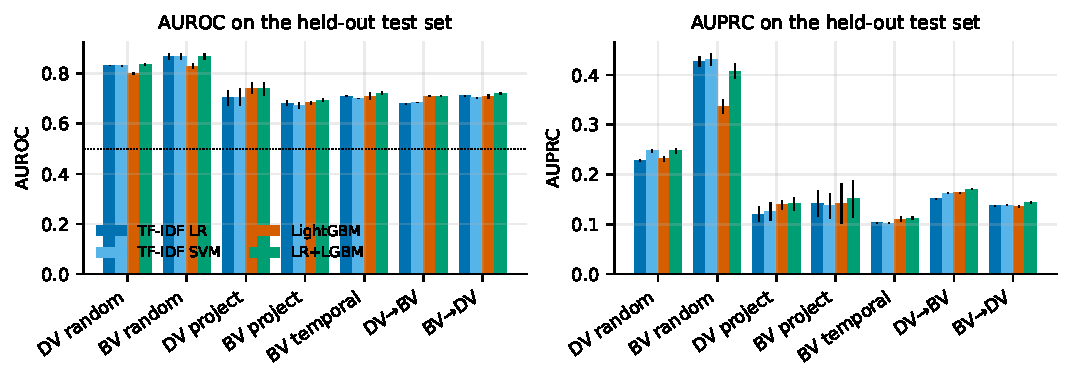
\includegraphics[width=\linewidth]{figs/fig_detection.pdf}
\caption{Detection performance of the four scorers across the seven scenarios (mean $\pm$ s.d.\ over 3 seeds).}\label{fig:detection}
\end{figure}
\begin{table}[t]
\centering\small
\caption{Detection performance on the held-out test sets (mean $\pm$ s.d.\ over 3 seeds; best per row in bold). MCC uses the F1-optimal threshold chosen on ID calibration data.}\label{tab:detect}
\begin{tabular}{lcccc}
\toprule
Scenario & TF-IDF LR & TF-IDF SVM & LightGBM & LR+LGBM \\
\midrule
\multicolumn{5}{l}{\emph{Panel A: AUPRC}} \\
DV random & 0.229\,{\scriptsize$\pm$0.002} & \textbf{0.248\,{\scriptsize$\pm$0.003}} & 0.231\,{\scriptsize$\pm$0.004} & 0.248\,{\scriptsize$\pm$0.005} \\
BV random & 0.427\,{\scriptsize$\pm$0.010} & \textbf{0.432\,{\scriptsize$\pm$0.012}} & 0.337\,{\scriptsize$\pm$0.013} & 0.407\,{\scriptsize$\pm$0.015} \\
DV project & 0.120\,{\scriptsize$\pm$0.015} & 0.126\,{\scriptsize$\pm$0.018} & 0.139\,{\scriptsize$\pm$0.009} & \textbf{0.141\,{\scriptsize$\pm$0.013}} \\
BV project & 0.142\,{\scriptsize$\pm$0.027} & 0.137\,{\scriptsize$\pm$0.025} & 0.143\,{\scriptsize$\pm$0.040} & \textbf{0.151\,{\scriptsize$\pm$0.037}} \\
BV temporal & 0.103\,{\scriptsize$\pm$0.001} & 0.102\,{\scriptsize$\pm$0.000} & 0.110\,{\scriptsize$\pm$0.005} & \textbf{0.113\,{\scriptsize$\pm$0.003}} \\
DV$\to$BV & 0.151\,{\scriptsize$\pm$0.002} & 0.162\,{\scriptsize$\pm$0.001} & 0.163\,{\scriptsize$\pm$0.000} & \textbf{0.171\,{\scriptsize$\pm$0.001}} \\
BV$\to$DV & 0.137\,{\scriptsize$\pm$0.001} & 0.139\,{\scriptsize$\pm$0.001} & 0.136\,{\scriptsize$\pm$0.002} & \textbf{0.144\,{\scriptsize$\pm$0.002}} \\
\midrule
\multicolumn{5}{l}{\emph{Panel B: AUROC}} \\
DV random & 0.832\,{\scriptsize$\pm$0.001} & 0.832\,{\scriptsize$\pm$0.002} & 0.800\,{\scriptsize$\pm$0.002} & \textbf{0.836\,{\scriptsize$\pm$0.002}} \\
BV random & \textbf{0.869\,{\scriptsize$\pm$0.013}} & 0.867\,{\scriptsize$\pm$0.012} & 0.830\,{\scriptsize$\pm$0.010} & 0.869\,{\scriptsize$\pm$0.012} \\
DV project & 0.704\,{\scriptsize$\pm$0.030} & 0.706\,{\scriptsize$\pm$0.033} & \textbf{0.742\,{\scriptsize$\pm$0.022}} & 0.740\,{\scriptsize$\pm$0.026} \\
BV project & 0.683\,{\scriptsize$\pm$0.012} & 0.674\,{\scriptsize$\pm$0.012} & 0.684\,{\scriptsize$\pm$0.006} & \textbf{0.694\,{\scriptsize$\pm$0.005}} \\
BV temporal & 0.710\,{\scriptsize$\pm$0.002} & 0.701\,{\scriptsize$\pm$0.001} & 0.710\,{\scriptsize$\pm$0.013} & \textbf{0.722\,{\scriptsize$\pm$0.006}} \\
DV$\to$BV & 0.679\,{\scriptsize$\pm$0.001} & 0.685\,{\scriptsize$\pm$0.001} & \textbf{0.711\,{\scriptsize$\pm$0.003}} & 0.710\,{\scriptsize$\pm$0.002} \\
BV$\to$DV & 0.711\,{\scriptsize$\pm$0.001} & 0.704\,{\scriptsize$\pm$0.002} & 0.709\,{\scriptsize$\pm$0.006} & \textbf{0.721\,{\scriptsize$\pm$0.003}} \\
\midrule
\multicolumn{5}{l}{\emph{Panel C: MCC}} \\
DV random & \textbf{0.292\,{\scriptsize$\pm$0.004}} & 0.291\,{\scriptsize$\pm$0.006} & 0.257\,{\scriptsize$\pm$0.002} & 0.288\,{\scriptsize$\pm$0.006} \\
BV random & \textbf{0.415\,{\scriptsize$\pm$0.013}} & 0.413\,{\scriptsize$\pm$0.018} & 0.319\,{\scriptsize$\pm$0.011} & 0.387\,{\scriptsize$\pm$0.014} \\
DV project & 0.120\,{\scriptsize$\pm$0.025} & 0.134\,{\scriptsize$\pm$0.024} & 0.163\,{\scriptsize$\pm$0.030} & \textbf{0.165\,{\scriptsize$\pm$0.030}} \\
BV project & 0.112\,{\scriptsize$\pm$0.032} & 0.109\,{\scriptsize$\pm$0.036} & 0.125\,{\scriptsize$\pm$0.052} & \textbf{0.133\,{\scriptsize$\pm$0.057}} \\
BV temporal & 0.071\,{\scriptsize$\pm$0.011} & 0.073\,{\scriptsize$\pm$0.008} & 0.119\,{\scriptsize$\pm$0.007} & \textbf{0.121\,{\scriptsize$\pm$0.016}} \\
DV$\to$BV & 0.150\,{\scriptsize$\pm$0.007} & 0.161\,{\scriptsize$\pm$0.004} & 0.158\,{\scriptsize$\pm$0.005} & \textbf{0.166\,{\scriptsize$\pm$0.002}} \\
BV$\to$DV & 0.138\,{\scriptsize$\pm$0.002} & 0.146\,{\scriptsize$\pm$0.007} & 0.140\,{\scriptsize$\pm$0.006} & \textbf{0.149\,{\scriptsize$\pm$0.007}} \\
\bottomrule
\end{tabular}
\end{table}


\paragraph{AUROC is a poor proxy for operational value}
By Lemma~\ref{lem:auc}, AUROC averages the clearable fraction of benign functions over all miss budgets. A team that wants at most $5\%$ of vulnerabilities cleared by the tool uses only the left tail. Across the 84 scorer--scenario--seed combinations, the Spearman correlation between AUROC and the share of functions that can be cleared at $\alpha=5\%$ is only $\rho=0.38$. Within a scenario, scorers whose mean AUROC differs by $0.02$--$0.04$ differ by $0.04$--$0.13$ in clearable share (e.g.\ DiverseVul random: AUROC range $0.036$, SAR range $0.114$). Model selection for triage must therefore use the operating point of interest, not a global ranking metric.

\paragraph{A formatting shortcut in the Big-Vul release} While preparing the pre-trained-model experiment (Section~\ref{sec:rq6}) we found that the raw text of the Hugging Face release of Big-Vul carries a strong formatting signal: a classifier that sees only 15 formatting statistics (indentation, trailing whitespace, comment markers, line lengths; Table~\ref{tab:format}) reaches AUROC $0.919$ on a random split, higher than every semantic model in this paper (the raw-text CodeBERT ensemble of Section~\ref{sec:rq6}, which also sees the formatting, comes close at $0.893$), and whitespace structure alone (tabs, leading and trailing whitespace, indentation, brace placement) reaches $0.892$ against $0.687$ for size alone (Table~\ref{tab:formatabl}). The signal is present in PrimeVul as well (whitespace structure alone $0.841$) but not in DiverseVul, where size dominates ($0.719$ for size alone, $0.682$ for whitespace). All detectors in Sections~\ref{sec:rq1}--\ref{sec:rq5} operate on comment-stripped, whitespace-insensitive tokens and code metrics, and removing the only size-sensitive metrics (characters, lines, tokens) changes the AUROC of the LightGBM scorer by at most $0.006$ ($0.820\to0.818$ on Big-Vul, $0.801\to0.802$ on DiverseVul, $0.820\to0.814$ on PrimeVul), so the main results are not driven by it (the same holds on PrimeVul, Section~\ref{sec:rq8}); but results obtained by models that read raw Big-Vul text should be interpreted with this in mind.

\subsection{RQ2: Calibration is acceptable in-distribution and degrades under shift}\label{sec:rq2}
Table~\ref{tab:calib} reports ECE. Raw probabilities are mildly miscalibrated even on random splits (LR: $0.015$--$0.032$; LightGBM: $0.0075$--$0.018$), largely because training keeps at most 150\,000 benign functions. Platt scaling and isotonic regression fitted on ID calibration data reduce ECE to $0.004$--$0.015$ on random splits, but under shift the residual error is much larger: $0.014$--$0.030$ (LR and LightGBM, Platt scaling and isotonic regression) for the project, temporal and cross-dataset settings, i.e.\ roughly $30$--$60\%$ of the 5\% base rate, and the two methods perform alike. The one exception is LightGBM trained on DiverseVul and tested on Big-Vul, where raw probabilities ($0.008$) beat recalibrated ones ($0.018$). Importantly, because the clearance rule depends only on the ranking of scores, post-hoc calibration changes \emph{no} triage decision; calibration matters for reporting probabilities and for cost-based decisions, not for the miss-rate guarantee.
\begin{table}[t]
\centering\footnotesize
\caption{Expected calibration error (ECE, lower is better) on the test sets; Platt scaling and isotonic regression are fitted on ID calibration data. Mean over 3 seeds.}\label{tab:calib}
\resizebox{\linewidth}{!}{\begin{tabular}{lcccccc}
\toprule
Scenario & LR raw & LR Platt & LR isotonic & LGBM raw & LGBM Platt & LGBM isotonic \\
\midrule
DV random & 0.032 & 0.015 & 0.006 & 0.018 & 0.006 & 0.004 \\
BV random & 0.015 & 0.004 & 0.004 & 0.008 & 0.005 & 0.004 \\
DV project & 0.026 & 0.010 & 0.017 & 0.009 & 0.005 & 0.008 \\
BV project & 0.037 & 0.022 & 0.023 & 0.025 & 0.022 & 0.023 \\
BV temporal & 0.022 & 0.015 & 0.016 & 0.016 & 0.016 & 0.016 \\
DV$\to$BV & 0.031 & 0.020 & 0.021 & 0.008 & 0.018 & 0.018 \\
BV$\to$DV & 0.035 & 0.023 & 0.026 & 0.022 & 0.022 & 0.023 \\
\bottomrule
\end{tabular}}
\end{table}


\subsection{RQ3: The miss-rate guarantee holds under exchangeability and fails under shift}\label{sec:rq3}

\paragraph{Validity on exchangeable splits}
Figure~\ref{fig:validity} (left) and Table~\ref{tab:alpha} show that on random splits the realised miss rate matches the nominal budget: at $\alpha=10\%$ it is $10.1\%$ (DiverseVul) and $8.6\%$ (Big-Vul); over all budgets and seeds the excess over $\alpha$ is $-0.4$ percentage points on average (one-sided Wilcoxon $p=0.80$ for ``exceeds''), and the realised-to-nominal ratio is $0.96$. This confirms Proposition~\ref{prop:valid} on real detector scores. At this budget the rule clears $54$--$55\%$ of all functions (SAR; Figure~\ref{fig:sar}), i.e.\ it reduces the number of functions that must be reviewed per 1\,000 from $1000$ to about $450$.

\begin{figure}[t]
\centering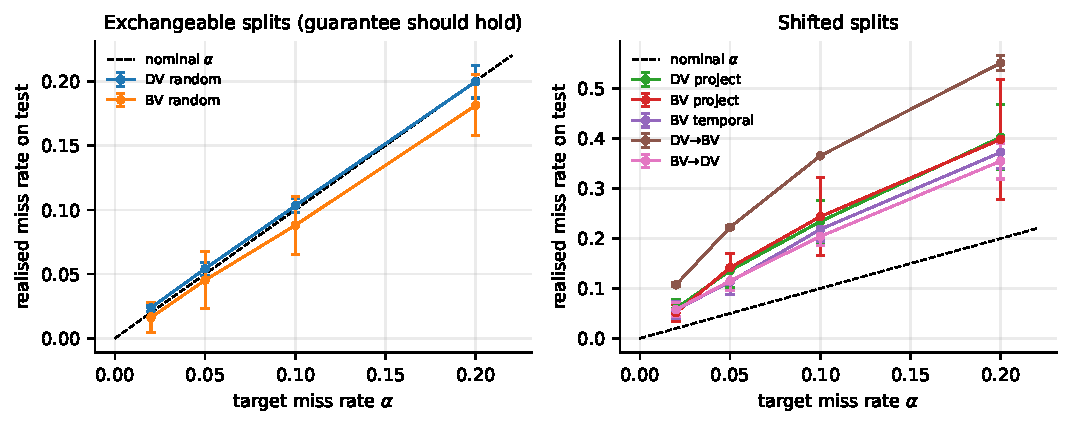
\includegraphics[width=\linewidth]{figs/fig_validity.pdf}
\caption{Realised versus nominal miss rate for source-calibrated conformal clearance (LR+LGBM scorer; mean $\pm$ s.d.\ over seeds). The dashed line is the target.}\label{fig:validity}
\end{figure}

\paragraph{Failure under shift}
In every shifted scenario the guarantee is violated (Figure~\ref{fig:validity}, right). At $\alpha=10\%$ the realised miss rate is $24.0\%$ (Big-Vul project), $23.6\%$ (DiverseVul project), $21.7\%$ (Big-Vul temporal), $20.3\%$ (Big-Vul$\to$DiverseVul) and $37.0\%$ (DiverseVul$\to$Big-Vul), on average $2.7\times$ the budget (excess $+12.8$ points, $p<10^{-11}$). At $\alpha=2\%$ the miss rates are $5.0$--$10.7\%$. The severity of the project-level violation depends on which projects are held out: for Big-Vul project the realised miss rate at $\alpha=10\%$ is $16.9$, $32.0$ and $23.0\%$ in the three partitions (and $9.4$, $17.7$ and $3.0\%$ in the three partitions of the subsample used in Section~\ref{sec:rq6}, for the normalised CodeBERT ensemble, where it can even fall below the nominal level), whereas the temporal and cross-dataset violations are stable across seeds ($20.1$--$24.2\%$, $18.3$--$22.0\%$, and $36.7$--$37.2\%$). Project shift is thus a high-variance threat, temporal and dataset shift a consistent one. Meanwhile the SAR reported for the invalid rule is deceptively high ($47.6$--$66.1\%$, Table~\ref{tab:guar}), so a team calibrating on a convenient hold-out would believe the tool is both safe and efficient.
Proposition~\ref{prop:shift} bounds the excess by the KS distance between the scores of calibration and test positives; Figure~\ref{fig:ks} shows that all $336$ (scenario, seed, scorer, $\alpha$) points lie below the bound. The excess is strongly related to the shift ($\rho=0.74$). The bound is conservative in typical cases (the KS distance is a median $3.1\times$ the excess, inter-quartile range $1.9$--$6.2$) but nearly tight in the worst one (excess up to $95\%$ of the KS distance), so it is a safe diagnostic, usable only if some labelled target positives exist.

\begin{figure}[t]
\centering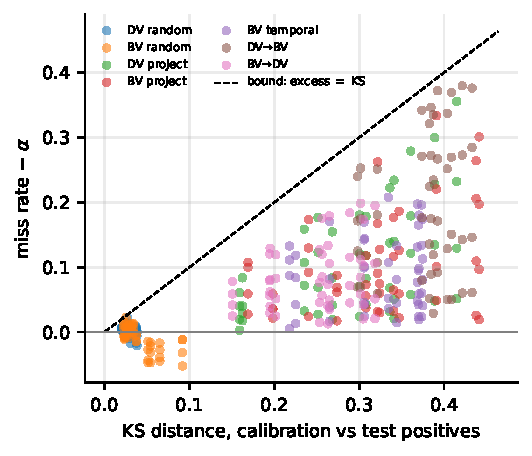
\includegraphics[width=.62\linewidth]{figs/fig_ks_bound.pdf}
\caption{Excess miss rate over the nominal budget versus the KS distance between calibration and test positive scores, for all scorers, budgets and seeds (336 points). All points lie below the diagonal bound of Proposition~\ref{prop:shift}.}\label{fig:ks}
\end{figure}
\begin{table}[t]
\centering\small
\caption{Realised miss rate (\%, mean $\pm$ s.d.\ over seeds) of the conformal clearance rule calibrated on source-distribution (ID) data, for four nominal budgets $\alpha$ (LR+LGBM scorer).}\label{tab:alpha}
\begin{tabular}{lcccc}
\toprule
Scenario & $\alpha{=}2\%$ & $\alpha{=}5\%$ & $\alpha{=}10\%$ & $\alpha{=}20\%$ \\
\midrule
DV random & 2.4{\scriptsize$\pm$0.2} & 5.5{\scriptsize$\pm$0.5} & 10.1{\scriptsize$\pm$0.6} & 19.8{\scriptsize$\pm$1.7} \\
BV random & 1.5{\scriptsize$\pm$1.2} & 4.6{\scriptsize$\pm$2.5} & 8.6{\scriptsize$\pm$2.3} & 18.2{\scriptsize$\pm$2.3} \\
DV project & 5.9{\scriptsize$\pm$1.6} & 13.8{\scriptsize$\pm$3.0} & 23.6{\scriptsize$\pm$3.8} & 40.5{\scriptsize$\pm$6.5} \\
BV project & 5.0{\scriptsize$\pm$1.6} & 13.5{\scriptsize$\pm$2.1} & 24.0{\scriptsize$\pm$7.6} & 39.8{\scriptsize$\pm$12.5} \\
BV temporal & 5.6{\scriptsize$\pm$1.1} & 11.5{\scriptsize$\pm$3.0} & 21.7{\scriptsize$\pm$2.2} & 37.4{\scriptsize$\pm$3.2} \\
DV$\to$BV & 10.7{\scriptsize$\pm$0.6} & 22.4{\scriptsize$\pm$0.3} & 37.0{\scriptsize$\pm$0.3} & 55.3{\scriptsize$\pm$1.6} \\
BV$\to$DV & 5.9{\scriptsize$\pm$1.6} & 11.2{\scriptsize$\pm$2.0} & 20.3{\scriptsize$\pm$1.9} & 35.8{\scriptsize$\pm$3.4} \\
\bottomrule
\end{tabular}
\end{table}


\paragraph{Remedies}
Table~\ref{tab:guar} and Figure~\ref{fig:recal} compare the remedies at $\alpha=10\%$.
\emph{Covariate-shift weighting} helps in two scenarios (DiverseVul project: $23.6\to15.1\%$; DiverseVul$\to$Big-Vul: $37.0\to14.9\%$) but not in the other three (Big-Vul project $24.0\to18.6\%$, Big-Vul temporal $21.7\to22.6\%$, Big-Vul$\to$DiverseVul $20.3\to19.5\%$); on these two corpora it never restores the budget. The estimated weights are extremely skewed: the cap of 20 is reached for $22\%$ of the Big-Vul test functions in DiverseVul$\to$Big-Vul and for $15\%$ in Big-Vul project (median test weight $5.5$ and $5.4$ against calibration weights around $0.2$--$0.3$), so a few calibration positives carry most of the weight and the effective calibration size is small; together with a probably violated covariate-shift assumption for code, this explains why weighting is not a reliable repair.
\emph{Recalibration on labelled target positives} restores the budget: with $k=100$ the realised miss rate is $9.2$--$13.0\%$ across the five shifted scenarios (four of the five scenarios are within $10\%\pm0.8$ points; Big-Vul project is high at $13.0\%$), with a SAR of $26.7$--$31.8\%$; $k=50$ already gives $9.2$--$12.1\%$, and $k=25$ is conservative ($7.3$--$9.6\%$) because the finite-sample correction clears only $\lfloor0.1\cdot26\rfloor=2$ order statistics. The empirical curves fall inside the Beta band predicted by Corollary~\ref{cor:beta}, except for Big-Vul project at $k\ge200$, which stays slightly above it ($13.4\%$ against an upper band edge of about $12.6\%$), possibly because the projects of the target pool and of the test set differ. Because the guarantee is in expectation, the frequency with which a single calibration draw exceeds $\alpha+2$ points is $16$--$68\%$ at $k=100$; the PAC variant (Proposition~\ref{prop:pac}) cuts this to $\le7\%$ in all scenarios (mostly $\le2.3\%$), at the price of a lower SAR ($15.9$--$22.4\%$). The valid operating points under shift thus clear about $27$--$32\%$ of functions (non-PAC) or $16$--$22$\% (PAC), roughly half and a third of the $54$--$55\%$ available on random splits. Importantly, the PAC rule calibrated on \emph{source} data remains invalid under shift ($94$--$100\%$ violations), which confirms that the issue is exchangeability and not the choice of the quantile.

\begin{figure}[t]
\centering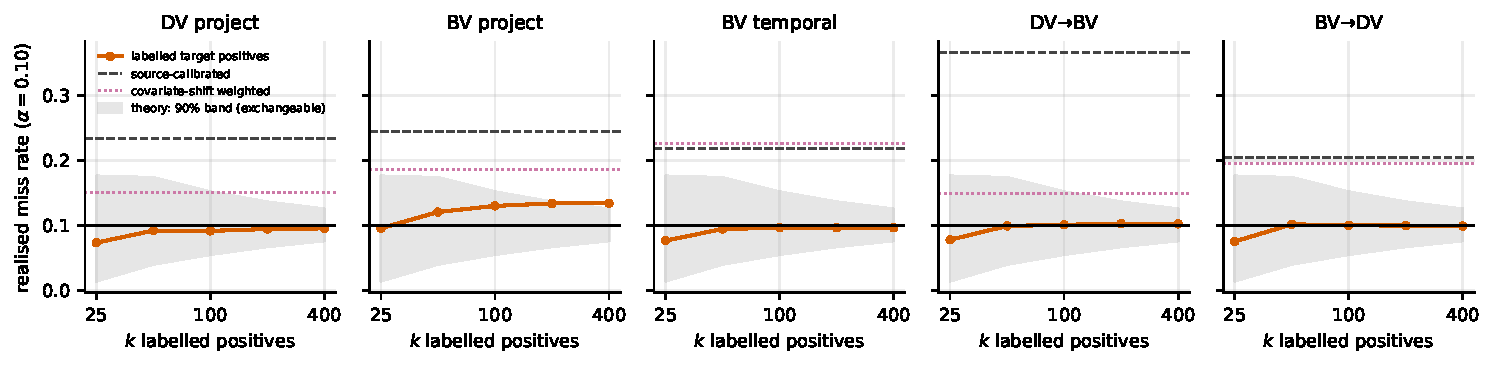
\includegraphics[width=\linewidth]{figs/fig_recalibration.pdf}
\caption{Realised miss rate at $\alpha=10\%$ as a function of the number $k$ of labelled target positives used for calibration (LR+LGBM scorer; mean over seeds). The shaded area is the 90\% band of Corollary~\ref{cor:beta} for exchangeable data; dashed and dotted lines are the source-calibrated and weighted rules.}\label{fig:recal}
\end{figure}
\begin{table}[t]
\centering\footnotesize
\caption{Conformal clearance at $\alpha{=}10\%$ (LR+LGBM scorer; all figures in \%). ID: calibrated on source data; Wtd: covariate-shift weighted; $k{=}100$: calibrated on 100 labelled target positives; PAC: $k{=}100$ with the high-probability rule ($\delta{=}0.1$) and its violation frequency $\Pr(M>\alpha+2\text{pp})$. A valid rule has miss $\lesssim10$.}\label{tab:guar}
\resizebox{\linewidth}{!}{\begin{tabular}{lccccccccc}
\toprule
Scenario & ID miss & ID SAR & Wtd miss & Wtd SAR & $k{=}100$ miss & $k{=}100$ SAR & PAC miss & PAC SAR & PAC viol. \\
\midrule
DV random & 10.1{\scriptsize$\pm$0.6} & 55.1 & -- & -- & -- & -- & -- & -- & -- \\
BV random & 8.6{\scriptsize$\pm$2.3} & 54.3 & -- & -- & -- & -- & -- & -- & -- \\
DV project & 23.6{\scriptsize$\pm$3.8} & 56.4 & 15.1 & 41.1 & 9.2 & 31.8 & 5.4 & 22.4 & 2 \\
BV project & 24.0{\scriptsize$\pm$7.6} & 47.6 & 18.6 & 34.5 & 13.0 & 28.1 & 6.9 & 15.9 & 7 \\
BV temporal & 21.7{\scriptsize$\pm$2.2} & 50.5 & 22.6 & 51.4 & 9.7 & 28.5 & 6.0 & 20.1 & 0 \\
DV$\to$BV & 37.0{\scriptsize$\pm$0.3} & 66.1 & 14.9 & 30.2 & 10.1 & 26.7 & 6.1 & 18.2 & 2 \\
BV$\to$DV & 20.3{\scriptsize$\pm$1.9} & 48.5 & 19.5 & 46.6 & 10.0 & 30.0 & 5.9 & 20.2 & 2 \\
\bottomrule
\end{tabular}}
\end{table}


\begin{figure}[t]
\centering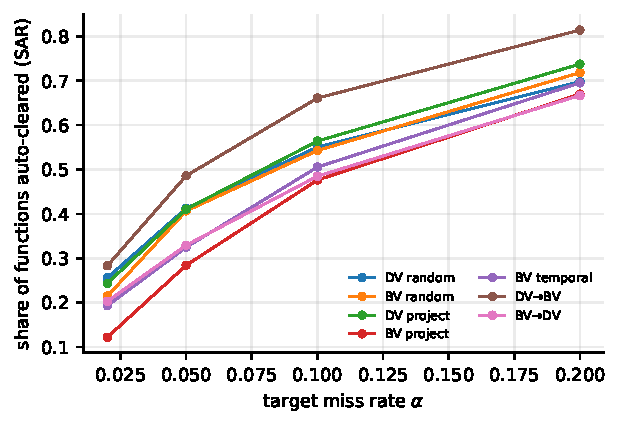
\includegraphics[width=.62\linewidth]{figs/fig_sar.pdf}
\caption{Share of functions that can be auto-cleared (SAR) versus nominal budget $\alpha$ for source-calibrated clearance (LR+LGBM). Values for shifted scenarios are \emph{not} valid; see Table~\ref{tab:guar}.}\label{fig:sar}
\end{figure}

\paragraph{Certified flagging}
Table~\ref{tab:flag} shows that the opposite decision, flagging with certified precision, offers little. With $\beta=50\%$ the Learn-then-Test procedure certifies a threshold that flags only $0.09\%$ (DiverseVul) and $2.6\%$ (Big-Vul) of the test functions on random splits (realised precision $80\%$ and $57\%$); for $\beta=70\%$ the flagged share is at most $0.3\%$ on random splits. Under shift the certification fails as well: for $\beta=50\%$, realised precision is $27\%$ (Big-Vul project), $19\%$ (Big-Vul temporal) and $23\%$ (Big-Vul$\to$DiverseVul), and the DiverseVul-trained detectors certify nothing. Learned detectors can \emph{clear} some code with a quantifiable risk, but at the precision available today they cannot be used to \emph{confirm} vulnerabilities for more than a few per cent of the code.
\begin{table}[t]
\centering\footnotesize
\caption{Certified auto-flagging (Learn-then-Test, $\delta{=}0.05$): share of test functions flagged (\%) and realised precision (\%); ``--'' = no threshold could be certified.}\label{tab:flag}
\resizebox{\linewidth}{!}{\begin{tabular}{lcccccc}
\toprule
Scenario & $\beta{=}.3$ flagged & prec. & $\beta{=}.5$ flagged & prec. & $\beta{=}.7$ flagged & prec. \\
\midrule
DV random & 1.35 & 41 & 0.09 & 80 & 0.02 & 78 \\
BV random & 8.06 & 33 & 2.57 & 57 & 0.30 & 87 \\
DV project & 0.16 & 39 & 0.00 & 43 & 0.00 & -- \\
BV project & 9.39 & 18 & 1.64 & 27 & 0.10 & 45 \\
BV temporal & 6.67 & 15 & 0.54 & 19 & 0.03 & 23 \\
DV$\to$BV & 0.33 & 56 & 0.00 & 79 & 0.00 & 75 \\
BV$\to$DV & 11.25 & 16 & 3.02 & 23 & 0.71 & 27 \\
\bottomrule
\end{tabular}}
\end{table}


\subsection{RQ4: Accountability, robustness and explanations}\label{sec:rq4}

\paragraph{The marginal guarantee is very uneven across function sizes}
Table~\ref{tab:bucket} and Figure~\ref{fig:mondrian} show that, even on exchangeable splits where the marginal guarantee holds, the miss rate at $\alpha=10\%$ is $41.4\%$ for the shortest third of DiverseVul functions and $2.2\%$ for the longest third ($25.8\%$ versus $2.9\%$ in Big-Vul). Short functions that contain vulnerabilities look like the many short benign functions, so most of the budget is consumed there. Length-conditional (Mondrian) calibration (Proposition~\ref{prop:mondrian}) equalises the three groups ($10.8/12.0/9.4\%$ in DiverseVul and $8.0/10.5/8.2\%$ in Big-Vul) at the price of a lower overall SAR ($55.2\to44.2\%$ and $54.2\to45.6\%$). Under shift it narrows the gap (e.g.\ Big-Vul project: $85.8/53.8/10.4\%\to47.3/45.4/18.1\%$) but does not restore validity, as expected, since exchangeability remains violated.

\begin{figure}[t]
\centering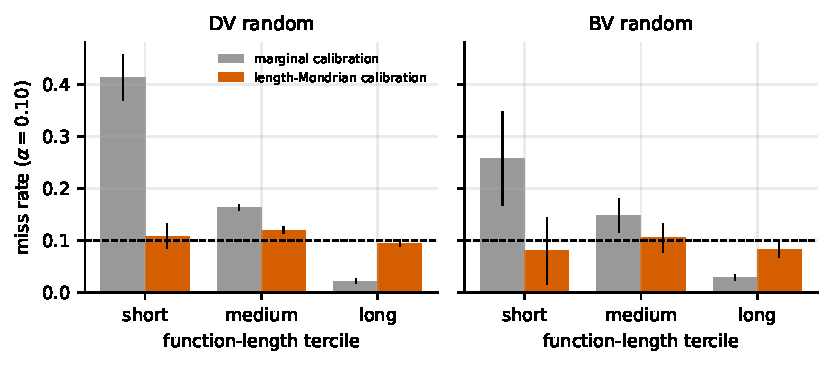
\includegraphics[width=.82\linewidth]{figs/fig_mondrian.pdf}
\caption{Miss rate per function-length tercile at $\alpha=10\%$ on random splits, marginal versus Mondrian calibration (LR+LGBM scorer, mean $\pm$ s.d.).}\label{fig:mondrian}
\end{figure}
\begin{table}[t]
\centering\footnotesize
\caption{Miss rate (\%) per function-length tercile at $\alpha{=}10\%$ for marginal (left) and Mondrian (right) calibration, with the overall share cleared (SAR). LR+LGBM scorer, ID calibration.}\label{tab:bucket}
\resizebox{\linewidth}{!}{\begin{tabular}{lcccccccc}
\toprule
Scenario & short & medium & long & SAR & short & medium & long & SAR \\
\midrule
DV random & 41.4 & 16.3 & 2.2 & 55.2 & 10.8 & 12.0 & 9.4 & 44.2 \\
BV random & 25.8 & 14.8 & 2.9 & 54.2 & 8.0 & 10.5 & 8.2 & 45.6 \\
DV project & 84.5 & 42.8 & 4.5 & 55.4 & 34.0 & 25.9 & 19.8 & 43.7 \\
BV project & 85.8 & 53.8 & 10.4 & 55.0 & 47.3 & 45.4 & 18.1 & 40.6 \\
BV temporal & 75.7 & 47.5 & 8.5 & 54.1 & 33.2 & 29.4 & 14.5 & 37.7 \\
DV$\to$BV & 90.5 & 51.3 & 7.8 & 57.1 & 37.5 & 33.5 & 29.1 & 45.2 \\
BV$\to$DV & 75.6 & 41.1 & 8.2 & 53.4 & 40.4 & 24.3 & 17.6 & 41.3 \\
\bottomrule
\end{tabular}}
\end{table}


\paragraph{Per-CWE disparity}
Figure~\ref{fig:cwe} reports miss rates per CWE for the classes with at least 15 vulnerable test functions. In DiverseVul, LightGBM misses $17.6\%$ of CWE-416 (use after free), $14.6\%$ of CWE-476 (NULL dereference) and $11.3\%$ of CWE-200, against $7.3\%$ for CWE-119, $6.8\%$ for CWE-125 and $9.1\%$ for CWE-787 (all at a nominal $10\%$); in Big-Vul the range among the most frequent classes is $2.6\%$ (CWE-125) to $14.9\%$ (CWE-264). The budget is therefore met on average but not per vulnerability class; classes that are reported separately (for audits, for example) need their own calibration, which requires sufficient labelled examples per class.
\begin{figure}[t]
\centering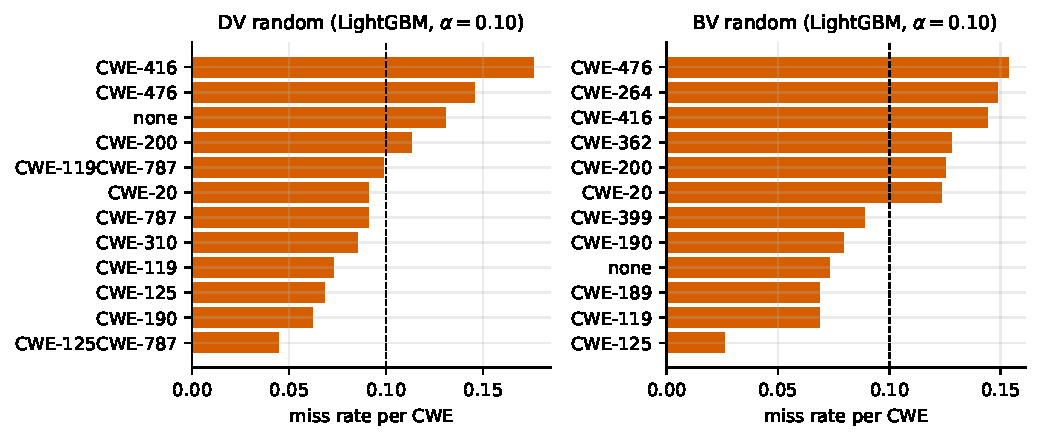
\includegraphics[width=\linewidth]{figs/fig_cwe.pdf}
\caption{Per-CWE miss rate at $\alpha=10\%$ on random splits (LightGBM, mean over seeds); the dashed line is the nominal budget.}\label{fig:cwe}
\end{figure}

\paragraph{Decision consistency under semantics-preserving rewrites}
Table~\ref{tab:robust} and Figure~\ref{fig:robust} show how the clear/review decision changes when functions are rewritten without changing behaviour. Renaming local identifiers flips $10.4\%$ of all decisions on average (and $5.6\%$ of the vulnerable functions) and inserting dead code $6.0\%$ ($2.6\%$); both together flip $13.5\%$ ($6.7\%$). The score ranking is largely preserved (Spearman $\rho=0.88$--$0.997$) and AUROC drops only by about $0.02$, but the miss rate moves from $8.6$--$11.3\%$ (original) to up to $13.5\%$ after renaming (LightGBM, DiverseVul), i.e.\ the nominal budget can be exceeded after cosmetic changes to the inputs (by $2.3$ points in the worst case, within about two points in the others). Because the triage threshold sits in the dense part of the score distribution, small score changes translate into many decision flips, which matters for accountability: the same code can be cleared or sent to review depending on variable names.
\begin{figure}[t]
\centering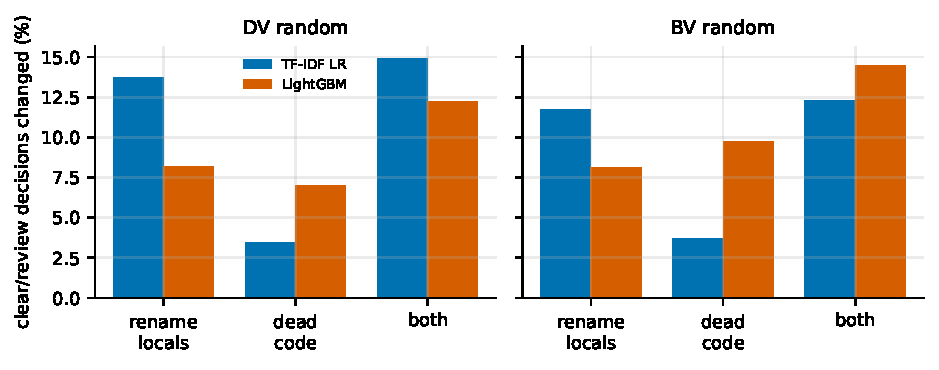
\includegraphics[width=.8\linewidth]{figs/fig_robust.pdf}
\caption{Share of clear/review decisions that change after each rewrite (5\,200 test functions per scenario, $\alpha=10\%$).}\label{fig:robust}
\end{figure}
\begin{table}[t]
\centering\footnotesize
\caption{Consistency of triage decisions ($\alpha{=}10\%$, ID calibration) on 1\,200 vulnerable and 4\,000 benign random test functions after semantics-preserving rewrites. ``Flipped'' = share of all (resp.\ vulnerable) functions whose clear/review decision changes.}\label{tab:robust}
\resizebox{\linewidth}{!}{\begin{tabular}{lllccccc}
\toprule
Scenario & Model & Rewrite & AUROC & Miss (\%) & Flipped (\%) & Flipped, vuln. (\%) & Spearman $\rho$ \\
\midrule
DV random & TF-IDF LR & original & 0.838 & 9.4 & 0.0 & 0.0 & 1.000 \\
DV random & TF-IDF LR & rename locals & 0.824 & 10.5 & 13.8 & 5.4 & 0.898 \\
DV random & TF-IDF LR & dead code & 0.837 & 8.4 & 3.5 & 1.3 & 0.997 \\
DV random & TF-IDF LR & both & 0.823 & 8.9 & 14.9 & 5.7 & 0.893 \\
DV random & LightGBM & original & 0.804 & 11.2 & 0.0 & 0.0 & 1.000 \\
DV random & LightGBM & rename locals & 0.788 & 13.5 & 8.2 & 6.8 & 0.937 \\
DV random & LightGBM & dead code & 0.800 & 9.4 & 7.0 & 3.2 & 0.978 \\
DV random & LightGBM & both & 0.785 & 10.1 & 12.2 & 8.2 & 0.917 \\
BV random & TF-IDF LR & original & 0.859 & 8.6 & 0.0 & 0.0 & 1.000 \\
BV random & TF-IDF LR & rename locals & 0.848 & 8.4 & 11.7 & 4.7 & 0.924 \\
BV random & TF-IDF LR & dead code & 0.860 & 10.5 & 3.7 & 1.9 & 0.994 \\
BV random & TF-IDF LR & both & 0.849 & 10.0 & 12.3 & 5.6 & 0.917 \\
BV random & LightGBM & original & 0.825 & 8.9 & 0.0 & 0.0 & 1.000 \\
BV random & LightGBM & rename locals & 0.810 & 10.9 & 8.1 & 5.7 & 0.937 \\
BV random & LightGBM & dead code & 0.820 & 8.3 & 9.7 & 3.9 & 0.945 \\
BV random & LightGBM & both & 0.804 & 10.0 & 14.5 & 7.2 & 0.879 \\
\bottomrule
\end{tabular}}
\end{table}


\paragraph{Explanations}
For the explanation analysis we use an interpretable LightGBM on the 71 named code metrics (Table~\ref{tab:explain}; AUROC $0.75$ on both random splits and $0.69$--$0.71$ on leak-free cross-dataset transfer, below the token-based scorers). TreeSHAP attributions are \emph{faithful} by deletion (Figure~\ref{fig:explain}, left): neutralising the ten highest-attributed features lowers the logit of the 10\% highest-scored functions by $1.63$ (DiverseVul) and $1.40$ (Big-Vul), versus $1.09$ and $0.67$ for the top-ten features by global gain and $-0.46$ and $-0.39$ for random features, so local attributions identify the features that drive the decision better than a global ranking does. They are also \emph{consistent}: the Spearman correlation of global importances is $0.97$ between training seeds and $0.90$ between a model trained on DiverseVul and one trained on Big-Vul. What they reveal is unflattering, however: the most important features are function size (characters, lines, tokens) and the number of parentheses (Figure~\ref{fig:explain}, right), i.e.\ the model largely predicts that longer, more complex functions are vulnerable. This is consistent with the length-dependent miss rate above and with the known confound that functions touched by security fixes tend to be larger. As a check on identifier shortcuts in the token model, we compared the 200 highest positive-weight lexical features of the DiverseVul logistic regression with frequency-matched random features: the former occur in a median of $11$ projects versus $13.5$ for the controls ($6\%$ versus $3\%$ occur in at most five projects), i.e.\ we do not find that the highest-weighted tokens are markedly more project-specific.
\begin{figure}[t]
\centering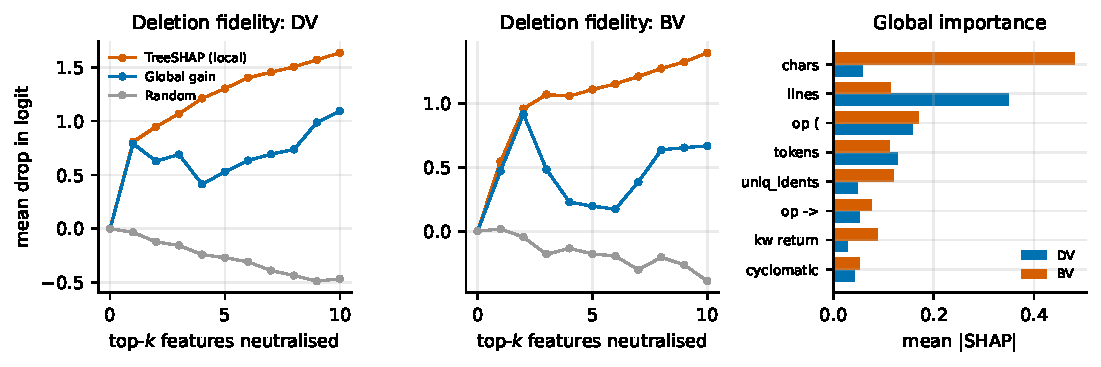
\includegraphics[width=\linewidth]{figs/fig_explain.pdf}
\caption{Explanation analysis for the metrics-only LightGBM. Left and centre: deletion fidelity (mean logit drop when the top-$k$ features of each function are neutralised). Right: mean $|$SHAP$|$ of the eight most important features.}\label{fig:explain}
\end{figure}
\begin{table}[t]
\centering\footnotesize
\caption{Interpretable metrics-only LightGBM used for the explanation analysis (3 seeds); cross-dataset rows exclude leaked functions.}\label{tab:explain}
\begin{tabular}{lcc}
\toprule
Train$\to$test & AUROC & AUPRC \\
\midrule
DV & 0.749\,{\scriptsize$\pm$0.002} & 0.164\,{\scriptsize$\pm$0.003} \\
BV & 0.756\,{\scriptsize$\pm$0.009} & 0.207\,{\scriptsize$\pm$0.012} \\
DV$\to$BV & 0.694\,{\scriptsize$\pm$0.001} & 0.132\,{\scriptsize$\pm$0.002} \\
BV$\to$DV & 0.710\,{\scriptsize$\pm$0.002} & 0.137\,{\scriptsize$\pm$0.002} \\
\bottomrule
\end{tabular}
\end{table}


\subsection{RQ5: Operational value}\label{sec:rq5}

\paragraph{Comparison with a rule-based analyser}
Flawfinder reports at least one hit for only $4.7$--$17.5\%$ of the functions and its scores barely rank the vulnerable functions (AUROC $0.535$--$0.611$, Table~\ref{tab:flaw}). Its only conservative policy, clearing functions without hits, auto-clears $82.5$--$95.3\%$ of the code but misses $62.9$--$89.8\%$ of the vulnerabilities. At the same clearance share the learned scorer misses $49.6$--$81.3\%$, and for the same (high) miss rate it could clear $84.7$--$98.8\%$ (Figure~\ref{fig:flaw}). Neither is useful as an unattended filter at those operating points; the contrast is that the learned scorer provides a whole curve from which a budget such as $10\%$ can be chosen and certified, whereas Flawfinder provides a single, uncontrolled point.
\begin{figure}[t]
\centering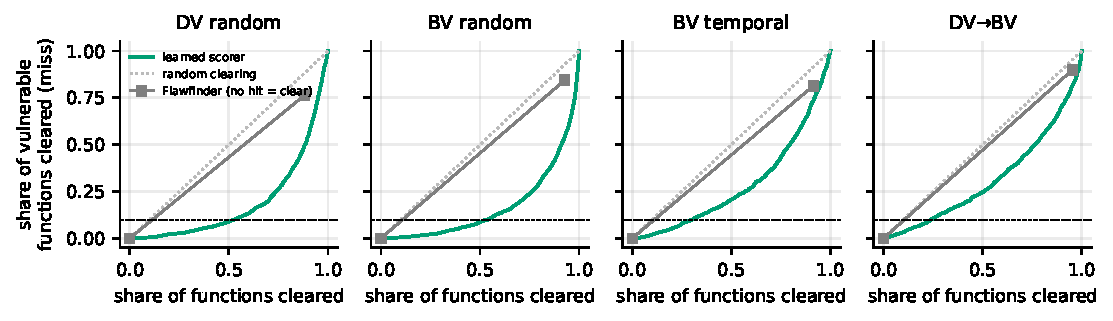
\includegraphics[width=\linewidth]{figs/fig_flaw.pdf}
\caption{Miss rate versus share of functions cleared for the learned scorer (curve) and Flawfinder (square; ``no hit $=$ clear''). Dashed: $10\%$ budget; dotted: random clearing.}\label{fig:flaw}
\end{figure}
\begin{table}[t]
\centering\footnotesize
\caption{Flawfinder (FF) versus the learned scorer (LR+LGBM rank average) on identical test functions (seed 0). The only conservative FF policy is to clear functions without any hit; its SAR and miss rate (\%) are compared with the learned scorer's miss rate at the same SAR and its SAR at the same miss rate.}\label{tab:flaw}
\resizebox{\linewidth}{!}{\begin{tabular}{lcccccccc}
\toprule
Scenario & AUROC FF & AUROC ML & AUPRC FF & AUPRC ML & FF SAR & FF miss & ML miss @SAR & ML SAR @miss \\
\midrule
DV random & 0.570 & 0.830 & 0.075 & 0.230 & 88.3 & 76.4 & 49.6 & 95.4 \\
BV random & 0.548 & 0.851 & 0.065 & 0.380 & 92.7 & 84.4 & 54.4 & 98.8 \\
DV project & 0.568 & 0.709 & 0.070 & 0.126 & 90.6 & 79.7 & 71.8 & 94.3 \\
BV project & 0.611 & 0.700 & 0.101 & 0.141 & 82.5 & 62.9 & 58.9 & 84.7 \\
BV temporal & 0.555 & 0.726 & 0.058 & 0.110 & 91.4 & 81.3 & 73.3 & 94.7 \\
DV$\to$BV & 0.535 & 0.697 & 0.066 & 0.163 & 95.3 & 89.8 & 81.3 & 98.4 \\
BV$\to$DV & 0.570 & 0.707 & 0.079 & 0.141 & 88.3 & 77.2 & 68.1 & 92.7 \\
\bottomrule
\end{tabular}}
\end{table}


\paragraph{Economic view}
Table~\ref{tab:cost} and Figure~\ref{fig:cost} apply the cost model of Eq.~\eqref{eq:cost} with $\alpha^\star$ chosen on ID calibration data. On random splits and for a missed vulnerability that costs $50$ reviews, the optimal budget is $\alpha^\star=0.07$--$0.09$, the rule clears $48$--$53\%$ of the code, and expected cost is $0.68$--$0.73$ of reviewing everything. Under project, temporal and cross-dataset shift the same procedure yields costs of $0.95$--$1.27$, i.e.\ no saving or a loss, because the miss rate it believes to have ($\approx\alpha^\star$) is far from the realised one. For $c_m=10$, triage appears to save $46$--$69\%$ of the cost but misses $35$--$75\%$ of the vulnerabilities, and for $c_m=200$ the saving is only $4$--$6\%$ on random splits and negative under shift; for $c_m=1000$ ``review everything'' is optimal in all scenarios. In short: delegation pays when a miss is worth tens, not hundreds, of reviews, and only if the miss rate is calibrated on the deployment distribution.
\begin{figure}[t]
\centering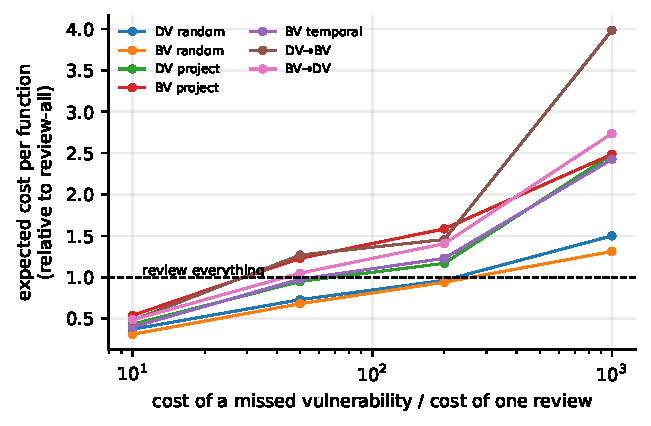
\includegraphics[width=.62\linewidth]{figs/fig_cost.pdf}
\caption{Expected cost per function relative to reviewing everything as a function of the cost ratio $c_m$ (LR+LGBM, $\alpha^\star$ selected on ID calibration data).}\label{fig:cost}
\end{figure}
\begin{table}[t]
\centering\footnotesize
\caption{Cost-optimal miss budget $\alpha^\star$ chosen on ID calibration data, its realised SAR (\%) and expected cost per function relative to reviewing everything ($=1$), for $c_m=10$, $50$, $200$ review units per missed vulnerability. LR+LGBM scorer.}\label{tab:cost}
\resizebox{\linewidth}{!}{\begin{tabular}{lccccccccc}
\toprule
Scenario & $\alpha^\star$ & SAR & cost & $\alpha^\star$ & SAR & cost & $\alpha^\star$ & SAR & cost \\
\midrule
DV random & 0.35 & 82 & 0.37 & 0.07 & 48 & 0.73 & 0.01 & 17 & 0.96 \\
BV random & 0.43 & 90 & 0.31 & 0.09 & 53 & 0.68 & 0.01 & 15 & 0.94 \\
DV project & 0.33 & 86 & 0.43 & 0.06 & 46 & 0.95 & 0.01 & 16 & 1.17 \\
BV project & 0.37 & 85 & 0.54 & 0.09 & 46 & 1.23 & 0.02 & 11 & 1.59 \\
BV temporal & 0.38 & 89 & 0.40 & 0.11 & 53 & 0.98 & 0.01 & 16 & 1.23 \\
DV$\to$BV & 0.38 & 93 & 0.48 & 0.08 & 62 & 1.27 & 0.01 & 17 & 1.46 \\
BV$\to$DV & 0.35 & 83 & 0.49 & 0.08 & 45 & 1.05 & 0.02 & 18 & 1.41 \\
\bottomrule
\end{tabular}}
\end{table}


\subsection{RQ6: Pre-trained code model and shortcut learning}\label{sec:rq6}
Tables~\ref{tab:cbdetect} and~\ref{tab:cbtriage} and Figure~\ref{fig:cb} report the CodeBERT experiment on the 30\,000-function subsample (Section~\ref{sec:design_cb}).

\paragraph{Raw text rewards a dataset artifact}
With raw text as input, CodeBERT looks excellent on Big-Vul: the CodeBERT ensemble reaches AUROC $0.893$ (random), $0.828$ (project) and $0.844$ (temporal), against $0.825$, $0.709$ and $0.728$ for the TF-IDF+LightGBM scorer trained on the same subsample. The formatting-only classifier (the 15 statistics above, of which whitespace structure alone carries most of the signal on Big-Vul) does even better ($0.924$, $0.895$, $0.909$; AUPRC $0.59$--$0.65$ against $0.12$--$0.25$ for the lexical scorers), and the advantage does not transfer: on DiverseVul the formatting-only classifier reaches $0.730$ (random) and $0.690$ (project), and Big-Vul$\to$DiverseVul falls to $0.627$ (Table~\ref{tab:cbdetect}). The artifact is visible in the data (Table~\ref{tab:format}): $3.0\%$ of the lines of vulnerable Big-Vul functions end in whitespace against $0.1\%$ of benign ones, $24.3\%$ versus $6.5\%$ of the functions start with whitespace, and vulnerable functions contain $2.9$ comment markers on average against $0.8$. It is much weaker in DiverseVul, which has other, smaller differences (comment markers $5.3$ versus $1.8$). When the same CodeBERT is given normalised text, its Big-Vul AUROC drops by $0.12$ in all three scenarios ($0.774$, $0.706$, $0.721$) while DiverseVul is unchanged ($0.753$ and $0.702$ versus $0.745$ and $0.698$).

\paragraph{Frozen CodeBERT adds little on normalised text}
Without the artifact, the CodeBERT ensemble is below the lexical scorer on random splits ($0.753$ vs.\ $0.790$ on DiverseVul, $0.774$ vs.\ $0.825$ on Big-Vul) and level under shift ($0.689$--$0.721$ vs.\ $0.701$--$0.728$). Combining the two (TF-IDF+CodeBERT) is the best normalised scorer in every shifted scenario, but by only $0.002$--$0.010$ AUROC (AUPRC $0.123$--$0.154$ vs.\ $0.115$--$0.148$). Frozen general-purpose embeddings thus do not change the picture of Section~\ref{sec:rq1}, and neither does fine-tuning (next paragraph).

\paragraph{Fine-tuning does not change the picture} Table~\ref{tab:ft} compares end-to-end fine-tuned CodeBERT (validation AUROC $0.76$--$0.83$) with the other scorers on exactly the same scenario--seed pairs (one or two seeds per scenario). Fine-tuning does not improve on the frozen embeddings (AUROC between $-0.015$ and $+0.009$ relative to the frozen ensemble) and stays $0.004$--$0.040$ below the lexical ensemble; combining it with the lexical scorers adds $0.000$--$0.015$ over the lexical ensemble alone. The triage findings are unchanged: with source calibration the realised miss rate at $\alpha=10\%$ is $10.9\%$ on the random splits (DiverseVul $10.4\%$, Big-Vul $11.5\%$, within the roughly one-point sampling error of one or two seeds) and $13.8\%$ on average over the shifted scenarios, from $10.2\%$ (Big-Vul project) to $20.7\%$ (DiverseVul$\to$Big-Vul), against $16.2\%$ for the lexical scorer and $14.6\%$ for frozen CodeBERT on the same pairs; recalibration on 100 labelled target positives restores $8.7$--$11.5\%$ at a SAR of $23$--$29\%$, and all $33$ observations satisfy the KS bound. The levels of automation that can be validly delegated are therefore driven by the shift and by the amount of labelled target data, not by the choice among these scorers.

\begin{figure}[t]
\centering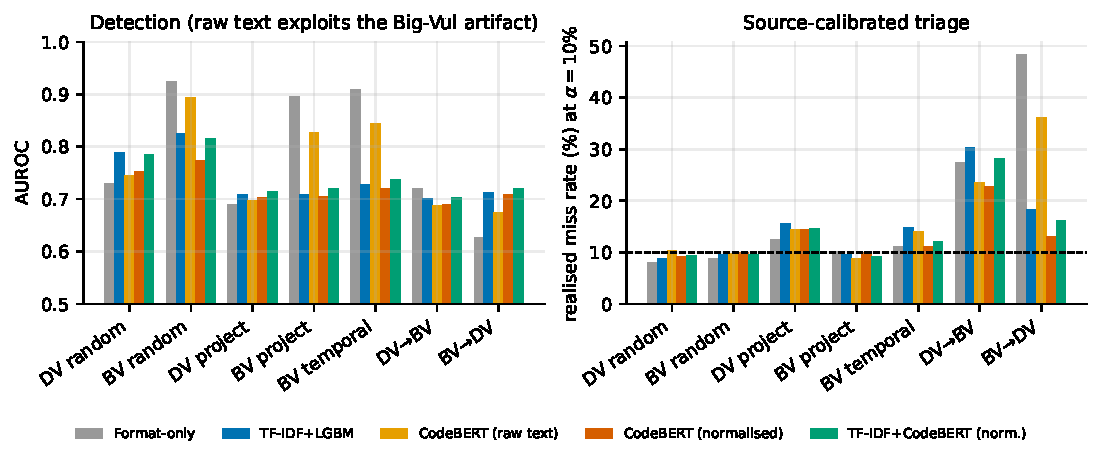
\includegraphics[width=\linewidth]{figs/fig_cb.pdf}
\caption{Left: AUROC of the formatting-only probe, the TF-IDF+LightGBM scorer and the CodeBERT scorers (raw and normalised text) on the subsample. Right: realised miss rate at $\alpha=10\%$ when calibrated on source data (dashed: nominal).}\label{fig:cb}
\end{figure}
\begin{table}[t]
\centering\footnotesize
\caption{Detection with frozen CodeBERT embeddings on the stratified subsample (mean over 3 seeds; AUPRC weighted to the true prevalence). Fmt: formatting-only classifier; CB raw / norm: CodeBERT on raw text / on comment-and-whitespace-normalised text; ensembles are standardised score sums.}\label{tab:cbdetect}
\resizebox{\linewidth}{!}{\begin{tabular}{lcccccccccc}
\toprule
Scenario & AUROC Fmt & AUROC TF-IDF & AUROC CB raw & AUROC CB norm & AUROC TF+CB & AUPRC Fmt & AUPRC TF-IDF & AUPRC CB raw & AUPRC CB norm & AUPRC TF+CB \\
\midrule
DV random & 0.730 & 0.790 & 0.745 & 0.753 & 0.784 & 0.143 & 0.208 & 0.168 & 0.167 & 0.203 \\
BV random & 0.924 & 0.825 & 0.893 & 0.774 & 0.816 & 0.651 & 0.251 & 0.445 & 0.180 & 0.240 \\
DV project & 0.690 & 0.708 & 0.698 & 0.702 & 0.715 & 0.122 & 0.137 & 0.122 & 0.135 & 0.147 \\
BV project & 0.895 & 0.709 & 0.828 & 0.706 & 0.719 & 0.588 & 0.142 & 0.312 & 0.142 & 0.152 \\
BV temporal & 0.909 & 0.728 & 0.844 & 0.721 & 0.737 & 0.647 & 0.115 & 0.291 & 0.121 & 0.123 \\
DV$\to$BV & 0.720 & 0.701 & 0.688 & 0.689 & 0.703 & 0.193 & 0.148 & 0.126 & 0.139 & 0.154 \\
BV$\to$DV & 0.627 & 0.712 & 0.674 & 0.709 & 0.721 & 0.101 & 0.147 & 0.113 & 0.140 & 0.153 \\
\bottomrule
\end{tabular}}
\end{table}

\begin{table}[t]
\centering\footnotesize
\caption{Fine-tuned CodeBERT on normalised text compared with the other scorers on exactly the same (scenario, seed) pairs (seed 0 for all scenarios, seed 1 additionally for BV-R, BV-P, BV-T and DV-R; the other models in Tables~\ref{tab:cbdetect} and~\ref{tab:cbtriage} use three seeds). AUROC, AUPRC (weighted to true prevalence) and realised miss rate (\%) of source-calibrated clearance at $\alpha{=}10\%$.}\label{tab:ft}
\resizebox{\linewidth}{!}{\begin{tabular}{lcccccccccccccc}
\toprule
Scenario & Seeds & AUROC TF-IDF+LGBM & AUROC CB frozen & AUROC CB fine-tuned & AUROC TF+CB-FT & AUPRC TF-IDF+LGBM & AUPRC CB frozen & AUPRC CB fine-tuned & AUPRC TF+CB-FT & miss TF-IDF+LGBM & miss CB frozen & miss CB fine-tuned & miss TF+CB-FT \\
\midrule
DV random & 2 & 0.787 & 0.754 & 0.747 & 0.787 & 0.200 & 0.169 & 0.163 & 0.202 & 8.9 & 9.4 & 10.4 & 9.2 \\
BV random & 2 & 0.827 & 0.780 & 0.789 & 0.833 & 0.250 & 0.181 & 0.208 & 0.266 & 9.5 & 9.4 & 11.5 & 10.6 \\
DV project & 1 & 0.716 & 0.702 & 0.692 & 0.722 & 0.136 & 0.134 & 0.118 & 0.140 & 14.3 & 13.3 & 18.5 & 14.6 \\
BV project & 2 & 0.693 & 0.687 & 0.689 & 0.708 & 0.134 & 0.135 & 0.129 & 0.140 & 11.7 & 13.6 & 10.2 & 10.6 \\
BV temporal & 2 & 0.728 & 0.720 & 0.723 & 0.739 & 0.115 & 0.117 & 0.115 & 0.123 & 14.4 & 11.0 & 11.0 & 13.4 \\
DV$\to$BV & 1 & 0.699 & 0.689 & 0.691 & 0.711 & 0.150 & 0.139 & 0.130 & 0.155 & 29.3 & 26.0 & 20.7 & 27.0 \\
BV$\to$DV & 1 & 0.712 & 0.711 & 0.696 & 0.720 & 0.146 & 0.135 & 0.128 & 0.149 & 18.0 & 13.5 & 14.7 & 18.9 \\
\bottomrule
\end{tabular}}
\end{table}

\begin{table}[t]
\centering\footnotesize
\caption{Formatting-shortcut audit on the stratified subsample (random 70/30 split). First two columns: LightGBM on 15 formatting features of the raw text only (indentation, trailing whitespace, comment markers, line lengths; AUPRC weighted to true prevalence). Next three: mean per function, vulnerable / benign. Last: AUROC of the main-study LightGBM with all metrics / with size-sensitive metrics (chars, lines, tokens) removed (seed 0).}\label{tab:format}
\resizebox{\linewidth}{!}{\begin{tabular}{lcccccc}
\toprule
Dataset & AUROC & AUPRC & Trailing-ws lines (\%) & Starts with ws (\%) & Comment markers & Main LGBM AUROC \\
\midrule
Big-Vul & 0.919 & 0.643 & 3.0 / 0.1 & 24.3 / 6.5 & 2.9 / 0.8 & 0.820 / 0.818 \\
DiverseVul & 0.721 & 0.145 & 0.5 / 0.2 & 4.2 / 7.9 & 5.3 / 1.8 & 0.801 / 0.802 \\
\bottomrule
\end{tabular}}
\end{table}


\paragraph{The guarantee findings replicate}
For every CodeBERT-based scorer the realised miss rate at $\alpha=10\%$ is on target on random splits (CodeBERT ensemble $9.6\%$ normalised, $10.0\%$ raw; TF-IDF $9.2\%$; combined $9.5\%$) and exceeded under shift (averages over the five shifted scenarios: $14.3\%$ normalised CodeBERT, $19.4\%$ raw CodeBERT, $17.7\%$ TF-IDF, $16.0\%$ combined; Table~\ref{tab:cbtriage}), and all $504$ (normalised) and $441$ (raw) observations satisfy the KS bound of Proposition~\ref{prop:shift}. Calibrating on 100 labelled target positives restores the budget for every scorer (mean miss $9.1$--$9.6\%$, range $7.5$--$10.1\%$ over scenarios), and the PAC variant keeps the violation frequency at or below $1.3\%$. The excess under shift is smaller than in the main study ($1.4$--$1.9\times$ against $2.7\times$) because of the smaller training sets and, above all, because the project partitions of the subsample are milder (see Section~\ref{sec:rq3}); the cross-dataset violation remains large ($22.7$--$30.4\%$ for DiverseVul$\to$Big-Vul).

\paragraph{A scorer can be valid and efficient for the wrong reason}
The shortcut scorers are the most efficient. Calibrated on 100 target positives, the formatting-only probe clears $62.4\%$ and $54.5\%$ of Big-Vul functions under project and temporal shift, and raw-text CodeBERT $53.8\%$ and $53.7\%$, against $27$--$32\%$ for the lexical scorers and $26.9$ and $26.1\%$ for normalised CodeBERT; within Big-Vul the formatting-only probe meets its budget with source calibration (miss $10.2\%$ and $11.1\%$ under project and temporal shift) and raw CodeBERT nearly so ($8.9\%$ and $14.0\%$). The same scorers break the moment the shortcut does not hold: calibrated on Big-Vul and applied to DiverseVul they miss $48.4\%$ (formatting-only) and $36.2\%$ (raw CodeBERT) of the vulnerabilities at a $10\%$ budget, against $13.0\%$ for normalised CodeBERT and $18.3\%$ for the lexical scorer. A conformal guarantee is a statement about the calibration distribution; it says nothing about whether the score separates vulnerabilities for a reason that survives deployment. This is one more reason to audit inputs for shortcuts and to calibrate on data from the deployment distribution.
\begin{table}[t]
\centering\footnotesize
\caption{Triage with CodeBERT scorers at $\alpha{=}10\%$ (\%). Left: realised miss rate when calibrated on source (ID) data; right: safe automation rate when calibrated on 100 labelled target positives (valid by Prop.~\ref{prop:valid}). Subsample experiment; see Table~\ref{tab:cbdetect} for column keys.}\label{tab:cbtriage}
\resizebox{\linewidth}{!}{\begin{tabular}{lcccccccccc}
\toprule
Scenario & miss Fmt & miss TF-IDF & miss CB raw & miss CB norm & miss TF+CB & SAR Fmt & SAR TF-IDF & SAR CB raw & SAR CB norm & SAR TF+CB \\
\midrule
DV random & 8.0 & 8.8 & 10.3 & 9.2 & 9.4 & -- & -- & -- & -- & -- \\
BV random & 8.9 & 9.6 & 9.7 & 10.0 & 9.5 & -- & -- & -- & -- & -- \\
DV project & 12.6 & 15.6 & 14.5 & 14.4 & 14.6 & 24.7 & 26.8 & 24.9 & 25.6 & 28.1 \\
BV project & 10.2 & 9.5 & 8.9 & 10.1 & 9.2 & 62.7 & 32.1 & 53.8 & 27.0 & 29.6 \\
BV temporal & 11.1 & 14.9 & 14.0 & 11.2 & 12.1 & 54.7 & 27.4 & 53.7 & 25.0 & 27.3 \\
DV$\to$BV & 27.4 & 30.4 & 23.6 & 22.7 & 28.1 & 17.1 & 24.7 & 23.4 & 24.2 & 24.5 \\
BV$\to$DV & 48.4 & 18.3 & 36.2 & 13.0 & 16.1 & 14.7 & 28.9 & 24.2 & 29.1 & 31.0 \\
\midrule
Mean, random & 8.4 & 9.2 & 10.0 & 9.6 & 9.5 &  &  &  &  &  \\
Mean, shifted & 21.9 & 17.7 & 19.4 & 14.3 & 16.0 & 34.8 & 28.0 & 36.0 & 26.2 & 28.1 \\
\bottomrule
\end{tabular}}
\end{table}


\subsection{RQ7: Online calibration under drift}\label{sec:rq7}
Table~\ref{tab:online} and Figure~\ref{fig:online} show the effect of replaying the test sets as streams at $\alpha=10\%$.
\paragraph{Static calibration drifts out of budget.} The fixed threshold misses $21.7\%$ (Big-Vul temporal), $24.0\%$ and $23.6\%$ (Big-Vul and DiverseVul project streams), $37.0\%$ (DiverseVul$\to$Big-Vul) and $20.3\%$ (Big-Vul$\to$DiverseVul) of the vulnerable functions over the stream. Its worst window is worse still ($27$--$45\%$): in the temporal stream the rolling miss rate stays between $15$ and $35\%$ for the whole period (Figure~\ref{fig:online}, left), so the violation is not a transient at the start.
\paragraph{ACI restores the long-run budget with delayed feedback only.} With $\gamma=0.01$ the overall miss rate is $10.2\%$, $10.1\%$, $10.2\%$ and $10.1\%$ on the temporal, DiverseVul project, DiverseVul$\to$Big-Vul and Big-Vul$\to$DiverseVul streams and $11.5\%$ on the Big-Vul project stream, where abrupt project switches are the hardest case. The deterministic bound of Proposition~\ref{prop:online} holds in all $168$ runs (Table~\ref{tab:gamma}; it is conservative, about $9$ points on average at $\gamma=0.01$, while the observed deviations are at most $3$ points). Worst-window miss rates fall to $13$--$19\%$. The sliding-window recalibration is comparable but somewhat worse in overall miss ($9.8$--$13.1\%$) and needs stored target scores; combining it with ACI gives the closest match to the budget ($9.9$--$11.3\%$).
\paragraph{The price is automation, and it is the valid level.} Under shift ACI ($\gamma=0.01$) clears $22$--$29\%$ of the functions (static: $48$--$66\%$, but invalid), in line with the $27$--$32\%$ obtained by one-off recalibration with 100 labelled target positives in Section~\ref{sec:rq3}. On the stationary random streams ACI clears $54.0\%$ and $56.9\%$ at $10.0\%$ and $9.9\%$ miss, as the static rule does ($55.1\%$, $54.3\%$): adaptation does no harm where there is no drift. Large steps are counter-productive: $\gamma=0.05$ keeps the budget but reduces SAR by $4$--$16$ points relative to $\gamma=0.01$, because its level oscillates; $\gamma\in[0.005,0.01]$ was best here.
\begin{figure}[t]
\centering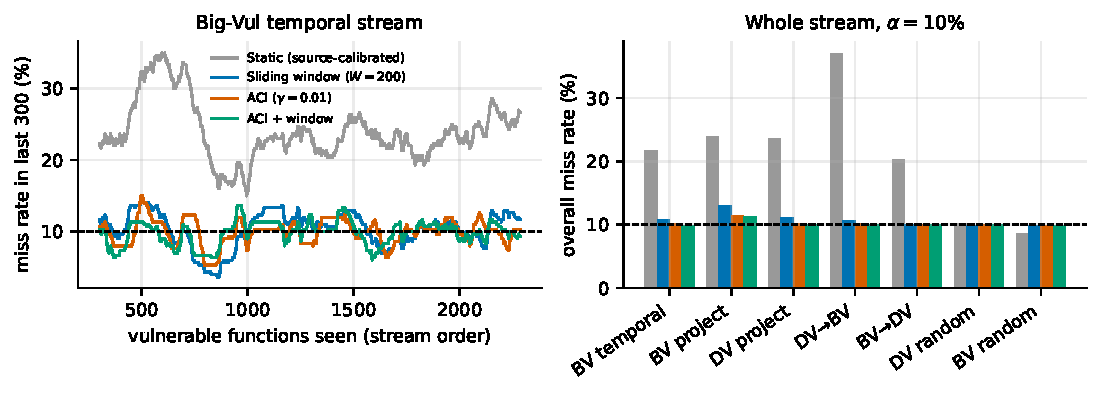
\includegraphics[width=\linewidth]{figs/fig_online.pdf}
\caption{Left: miss rate over the last 300 vulnerable functions along the Big-Vul temporal stream (seed 0, $\alpha=10\%$). Right: overall miss rate of each stream for the four policies (mean over 3 seeds).}\label{fig:online}
\end{figure}
\begin{table}[t]
\centering\footnotesize
\caption{Online risk control at $\alpha{=}10\%$ on arrival-ordered test streams (batches of 1\,000 functions, labels revealed after each batch; LR+LGBM scorer; mean over 3 seeds, \%). Overall miss rate over the stream, worst miss rate in any window of 300 vulnerable functions, and share of functions cleared (SAR). Static: threshold fixed from source calibration; SW: recalibrated on the last 200 observed vulnerable functions; ACI: adaptive conformal inference with step $\gamma$; ACI+window: ACI on the sliding-window reference.}\label{tab:online}
\resizebox{\linewidth}{!}{\begin{tabular}{lcccccccccccc}
\toprule
& \multicolumn{4}{c}{overall miss} & \multicolumn{4}{c}{worst window miss} & \multicolumn{4}{c}{SAR} \\
\cmidrule(lr){2-5}\cmidrule(lr){6-9}\cmidrule(lr){10-13}
Stream & Static & SW & ACI & ACI+W & Static & SW & ACI & ACI+W & Static & SW & ACI & ACI+W \\
\midrule
BV temporal & 21.7 & 10.8 & 10.2 & 9.9 & 32.8 & 15.9 & 13.8 & 14.1 & 50.5 & 30.2 & 29.2 & 27.3 \\
BV project & 24.0 & 13.1 & 11.5 & 11.3 & 30.0 & 16.7 & 17.0 & 16.7 & 47.6 & 28.3 & 22.4 & 22.7 \\
DV project & 23.6 & 11.2 & 10.1 & 10.0 & 33.8 & 17.7 & 18.7 & 19.2 & 56.4 & 34.4 & 29.4 & 27.1 \\
DV$\to$BV & 37.0 & 10.7 & 10.2 & 10.0 & 45.1 & 17.3 & 13.2 & 13.1 & 66.1 & 27.5 & 24.2 & 25.4 \\
BV$\to$DV & 20.3 & 10.0 & 10.1 & 10.0 & 27.0 & 16.0 & 13.0 & 13.1 & 48.5 & 30.2 & 29.1 & 28.5 \\
DV random & 10.1 & 9.8 & 10.0 & 10.0 & 14.1 & 13.3 & 13.1 & 13.1 & 55.1 & 53.7 & 53.9 & 49.7 \\
BV random & 8.6 & 9.8 & 9.9 & 9.9 & 11.2 & 12.9 & 12.7 & 12.9 & 54.3 & 57.3 & 56.9 & 52.8 \\
\bottomrule
\end{tabular}}
\end{table}

\begin{table}[t]
\centering\footnotesize
\caption{Sensitivity of ACI to the step size $\gamma$ ($\alpha{=}10\%$): overall miss, the deterministic bound $(1+\gamma b)/(\gamma N)$ of Proposition~\ref{prop:online} on its deviation from $\alpha$ (\%), SAR and worst-window miss.}\label{tab:gamma}
\begin{tabular}{lccccc}
\toprule
Stream & $\gamma$ & miss & bound & SAR & worst window \\
\midrule
BV temporal & 0.005 & 10.4 & 13.7 & 30.2 & 14.0 \\
BV temporal & 0.01 & 10.2 & 9.4 & 29.2 & 13.8 \\
BV temporal & 0.02 & 10.1 & 7.2 & 25.7 & 14.1 \\
BV temporal & 0.05 & 10.1 & 5.9 & 20.3 & 17.4 \\
BV project & 0.005 & 11.9 & 32.5 & 22.6 & 13.8 \\
BV project & 0.01 & 11.5 & 22.3 & 22.4 & 17.0 \\
BV project & 0.02 & 11.4 & 17.3 & 22.8 & 17.6 \\
BV project & 0.05 & 11.9 & 14.2 & 18.3 & 22.6 \\
DV$\to$BV & 0.005 & 10.4 & 6.5 & 26.0 & 15.2 \\
DV$\to$BV & 0.01 & 10.2 & 4.1 & 24.2 & 13.2 \\
DV$\to$BV & 0.02 & 10.2 & 2.9 & 20.6 & 15.6 \\
DV$\to$BV & 0.05 & 10.2 & 2.2 & 16.6 & 18.4 \\
\bottomrule
\end{tabular}
\end{table}


\subsection{RQ8: Replication on a third corpus (PrimeVul)}\label{sec:rq8}
\paragraph{Audit} PrimeVul contains 222\,558 clean functions (2.5\% vulnerable, 753 projects; Table~\ref{tab:data3}). It is not independent of the other two corpora: $77.3\%$ of its functions (171\,951) also occur in DiverseVul and $35.6\%$ (79\,323) in Big-Vul, including 4\,606 of its 5\,648 vulnerable functions that occur in DiverseVul. A cross-dataset evaluation between these corpora that does not remove shared functions would therefore mostly measure memorisation; all our cross-dataset scenarios do remove them.
\begin{table}[t]
\centering\footnotesize
\caption{Three corpora after normalisation and de-duplication. Pairwise overlaps of normalised functions: DiverseVul$\cap$Big-Vul 69,268 (42.7\% of Big-Vul), PrimeVul$\cap$DiverseVul 171,951 (77.3\% of PrimeVul), PrimeVul$\cap$Big-Vul 79,323 (35.6\% of PrimeVul).}\label{tab:data3}
\begin{tabular}{lrrrrr}
\toprule
Corpus & Raw & Exact duplicates & Clean & Vulnerable & Projects \\
\midrule
DiverseVul & 328,907 & 3,025 & 325,138 & 17,689 (5.4\%) & 800 \\
Big-Vul & 216,568 & 53,373 & 162,274 & 8,055 (5.0\%) & 309 \\
PrimeVul & 223,335 & 725 & 222,558 & 5,648 (2.5\%) & 753 \\
\bottomrule
\end{tabular}
\end{table}

\paragraph{Detection} With the same detectors (Table~\ref{tab:pv}), PrimeVul is the hardest corpus in absolute terms: AUROC $0.840$ and AUPRC $0.139$ on a random split ($5.5\times$ the prevalence of $2.5\%$), falling to $0.797$ and $0.111$ for held-out projects, $0.819$ and $0.114$ for later CVEs, and $0.715$--$0.826$ across the cross-dataset scenarios.
\paragraph{The guarantee replicates} On the random split the source-calibrated rule misses $10.7\%$ at $\alpha=10\%$. Under shift it misses more in all six scenarios: $11.8\%$ (temporal, the mildest), $13.2\%$ (DiverseVul$\to$PrimeVul), $14.0\%$ (Big-Vul$\to$PrimeVul), $19.0\%$ (project; $15.5$--$22.0\%$ across partitions), $23.9\%$ (PrimeVul$\to$DiverseVul) and $36.1\%$ (PrimeVul$\to$Big-Vul); the average over the shifted scenarios is $19.7\%$, i.e.\ $2.0\times$ the budget, and all $336$ observations satisfy the KS bound of Proposition~\ref{prop:shift}. Temporal shift is much less harmful here than on Big-Vul ($11.8$ against $21.7\%$), which shows that the size of the violation depends on the corpus and the split and cannot be inferred in advance. Covariate-shift weighting nearly restores the budget in three scenarios (project $19.0\to12.1\%$, temporal $11.8\to10.7\%$, DiverseVul$\to$PrimeVul $13.2\to10.6\%$), halves the excess for PrimeVul$\to$Big-Vul ($36.1\to19.5\%$) and does nothing for Big-Vul$\to$PrimeVul and PrimeVul$\to$DiverseVul ($14.1\%$, $23.1\%$): it is more useful here than on the other corpora but still not reliable. With 100 labelled target positives the realised miss rate is $8.7$--$10.7\%$ in every scenario, at a SAR of $25.9$--$50.8\%$ (PAC variant: $17.8$--$39.1\%$, violation frequency $\le4.5\%$ in all scenarios).
\paragraph{Shortcut} The raw-text formatting probe reaches AUROC $0.883$ on PrimeVul, of which whitespace structure alone gives $0.841$ and size alone $0.805$ (Table~\ref{tab:formatabl}); the scorers of this paper ignore whitespace, and removing the size-sensitive metrics changes the PrimeVul LightGBM AUROC by at most $0.006$. We did not trace the origin of the PrimeVul signal: because many benign functions are patched twins of vulnerable ones, formatting differences may reflect how the fixes were applied.
\begin{figure}[t]
\centering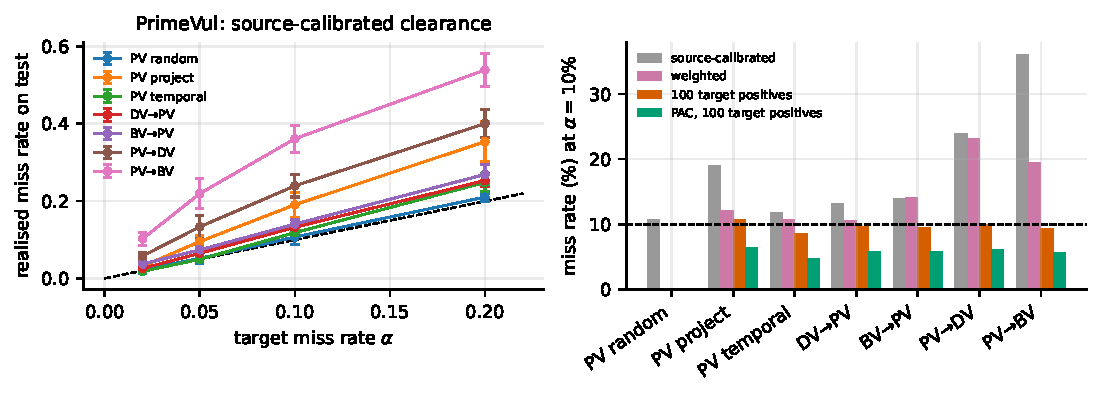
\includegraphics[width=\linewidth]{figs/fig_pv.pdf}
\caption{PrimeVul. Left: realised versus nominal miss rate of source-calibrated clearance (mean $\pm$ s.d.). Right: miss rate at $\alpha=10\%$ for source calibration, covariate-shift weighting and recalibration on 100 target positives (plain and PAC).}\label{fig:pv}
\end{figure}
\begin{table}[t]
\centering\footnotesize
\caption{Replication on PrimeVul (LR+LGBM scorer, mean over 3 seeds; \%, except AUROC/AUPRC). ID: source-calibrated clearance at $\alpha{=}10\%$; Wtd: covariate-shift weighted; $k{=}100$: calibrated on 100 labelled target positives; PAC: high-probability variant with its violation frequency. Cross-dataset scenarios exclude target functions that occur in the training corpus.}\label{tab:pv}
\resizebox{\linewidth}{!}{\begin{tabular}{lccccccccc}
\toprule
Scenario & AUROC & AUPRC & ID miss & ID SAR & Wtd miss & $k{=}100$ miss & $k{=}100$ SAR & PAC SAR & PAC viol. \\
\midrule
PV random & 0.840 & 0.139 & 10.7 & 57.6 & -- & -- & -- & -- & -- \\
PV project & 0.797 & 0.111 & 19.0 & 62.2 & 12.1 & 10.7 & 46.3 & 35.1 & 4.5 \\
PV temporal & 0.819 & 0.114 & 11.8 & 55.5 & 10.7 & 8.7 & 48.6 & 36.1 & 0.0 \\
DV$\to$PV & 0.826 & 0.123 & 13.2 & 58.5 & 10.6 & 9.7 & 50.8 & 39.1 & 1.7 \\
BV$\to$PV & 0.778 & 0.096 & 14.0 & 50.2 & 14.1 & 9.6 & 40.3 & 29.7 & 0.7 \\
PV$\to$DV & 0.735 & 0.199 & 23.9 & 55.2 & 23.1 & 10.0 & 31.5 & 22.4 & 2.0 \\
PV$\to$BV & 0.715 & 0.190 & 36.1 & 65.9 & 19.5 & 9.3 & 25.9 & 17.8 & 1.2 \\
\bottomrule
\end{tabular}}
\end{table}

\begin{table}[t]
\centering\footnotesize
\caption{Which formatting statistics carry the signal? AUROC of a LightGBM on groups of 15 raw-text statistics (random 70/30 split of a stratified sample): all, whitespace structure alone (tabs, carriage returns, trailing whitespace, leading whitespace, indentation, brace placement), size alone (characters, lines, mean line length), comment markers alone, and everything except whitespace structure.}\label{tab:formatabl}
\begin{tabular}{lccccc}
\toprule
Corpus & All & Whitespace only & Size only & Comments only & All but whitespace \\
\midrule
Big-Vul & 0.919 & 0.892 & 0.687 & 0.588 & 0.688 \\
DiverseVul & 0.721 & 0.682 & 0.719 & 0.658 & 0.718 \\
PrimeVul & 0.883 & 0.841 & 0.805 & 0.716 & 0.806 \\
\bottomrule
\end{tabular}
\end{table}


\section{Discussion}\label{sec:discussion}

\paragraph{What the results mean for practice}
The central message is operational: a detector's usefulness as a \emph{filter} is a property of the pair (detector, calibration data), not of the detector alone. Our findings translate into a short deployment recipe.
(1) \emph{Never calibrate the miss budget on a convenient hold-out of the training distribution when the tool is going to be used on other projects or later releases.} The resulting number is not conservative or optimistic by a small margin; it was off by a factor of 2.7 on average, and by 3.7 in the worst case.
(2) \emph{Budget for labelled data from the deployment distribution.} About $100$ labelled vulnerable functions from the target (the new project, or the latest release window) are enough to recover the nominal miss rate on average; $25$--$50$ are usable with a conservative finite-sample correction; with fewer than $\lceil1/\alpha\rceil-1$ labelled positives no clearance is possible at all.
(3) \emph{Choose between the expected and the high-probability guarantee.} The expected guarantee is exact but a single calibration draw exceeds the budget by two points in 16--68\% of the draws at $k=100$; the PAC rule brings this to $\le7\%$ for roughly $30\%$ less automation.
(4) \emph{Calibrate per group when the group is observable.} Function length was an easy and effective stratifier; per-class calibration would require more labelled data than most teams have.
(5) \emph{Monitor.} Every cleared function that later turns out to be vulnerable is a labelled event; Algorithm~\ref{alg:triage} re-calibrates on such events.
(6) \emph{Check the economics.} If a missed vulnerability is worth hundreds of reviews, delegating a share of the code to a detector of this quality does not pay off; if it is worth tens, the saving of $27$--$32\%$ at $c_m=50$ on exchangeable data turns into a change of between $+5\%$ and $-27\%$ (a loss) under shift when the budget is calibrated on source data.

\paragraph{What the results mean for research}
We suggest that evaluations of vulnerability detectors report, besides AUROC/F1, the \emph{miss-versus-clearance} curve at fixed budgets on shift-aware splits, together with a leakage audit. AUROC correlated only weakly with the clearable share at $\alpha=5\%$ ($\rho=0.38$) and the optimism of in-distribution validation reached a factor of 3.8 for AUPRC. The audit also shows that cross-dataset claims between these two corpora must remove shared functions: otherwise the reported AUPRC is $3.5$--$5.6\times$ too high. Finally, the negative result for covariate-shift weighting is informative: weighting is the standard shift remedy in the conformal literature, and for source code its assumptions (a stable conditional $\Pr(Y|x)$ and a well-estimated density ratio in a very high-dimensional token space) do not hold well enough in practice.

\paragraph{Relation to trustworthy automated software engineering}
The special-issue themes of transparency, accountability and governance appear here as concrete, testable artefacts: the miss budget is an auditable statement ("at most $\alpha$ of the vulnerabilities in the calibration distribution are cleared"), its failure under shift is detectable once any labelled outcomes exist, the unevenness across sizes and CWEs shows where the statement hides risk, and the consistency study shows that the decision, not only the score, must be assessed under benign input changes. The approach transfers to other automated decisions in the development pipeline, e.g.\ filtering of software-composition-analysis alerts, triage of AI-generated code for review, or deciding which dependencies need manual vetting, wherever a rare, costly event is missed silently and labelled outcomes arrive over time.

\paragraph{Limitations that shape how to read the results}
The size dependence found by the explanation analysis suggests that part of the predictive signal in these corpora is a size confound rather than vulnerability semantics, which is a data issue and not a triage issue, but it limits what any detector trained on them can deliver. Stronger detectors would raise the achievable automation but would not change the logic of Propositions~\ref{prop:valid} and~\ref{prop:shift}. Online variants that adapt the threshold over time are a natural extension for drift that is gradual rather than abrupt.

\section{Threats to validity}\label{sec:threats}

\paragraph{Construct validity}
Labels follow the datasets' convention: a function is vulnerable if it was modified by a vulnerability-fixing change, and benign otherwise. Benign functions may contain undiscovered flaws, and vulnerable ones may be mislabelled; label noise in such corpora is documented~\cite{croft2023data}. Our ``miss rate'' is therefore the miss rate with respect to these labels, and the true miss rate in deployment could be higher; the guarantee is only as meaningful as the calibration labels, which is why the monitoring step of Algorithm~\ref{alg:triage} matters. The publication year of a CVE is a proxy for the age of the code, and the CWE annotation is incomplete, which limits the per-CWE analysis to classes with at least 15 vulnerable test functions.
We remove exact duplicates after normalisation but not near-duplicates (clones with renamed identifiers or minor edits), so random-split numbers are probably still optimistic; this makes the contrast with the shifted scenarios conservative.
The semantics-preserving rewrites are implemented with lexical analysis rather than a compiler front-end; renaming is restricted to declared locals and parameters and was not validated by recompilation.

\paragraph{Internal validity}
Hyper-parameters are fixed across scenarios instead of being tuned per scenario, so absolute detection scores are lower than what careful tuning might reach; the triage conclusions concern the \emph{relationship} between nominal and realised miss rates, which does not depend on the absolute score. The realised miss rates are estimated on roughly 700--11\,200 vulnerable test functions per scenario and seed in the main study (about 750 in the CodeBERT subsample), giving a sampling error of about one percentage point at $\alpha=10\%$ in the smallest case; we use a two-point tolerance for violation counts and report standard deviations over three seeds. The conformal implementation is checked by a unit test against the $p$-value definition and by simulation of the finite-sample guarantee. The domain classifier behind the weighted variant is trained on the same features as the detector, and a better density-ratio estimator could do better, so the mixed result for weighting should be read as ``not reliably effective with standard estimators'' rather than ``never effective''. The online experiment replays static test sets as streams with complete, delayed labels, uses a single scorer (LR+LGBM), and the step size was compared post hoc on the same streams, so it shows what the method can achieve when misses are discovered, not how fast they are discovered in practice.

\paragraph{External validity}
We study three C/C++ corpora that share provenance (43\% of Big-Vul and 77\% of PrimeVul also occur in DiverseVul, Tables~\ref{tab:data} and~\ref{tab:data3}), so the cross-dataset scenarios are harder than a random split but not independent tests. Because the main experiments were designed to run on CPUs, we evaluate four lightweight detectors on the full corpora, and CodeBERT, frozen and fine-tuned, only on a 30\,000-function stratified subsample with the first 256 tokens (which truncates $34$--$44\%$ of the normalised functions) and, for fine-tuning, on one or two seeds because the GPU quota ended; larger or newer code models and large language models were not evaluated and may reach higher AUROC, although fine-tuned CodeBERT did not outperform the lexical scorers here. We expect the logic of our findings to hold, as the CodeBERT experiment suggests, but the conformal guarantee depends on exchangeability and not on the scorer, and the \emph{possibility} of a violation under shift follows from Proposition~\ref{prop:shift} (a diagnostic upper bound), while its size must be measured empirically, as the range from near-nominal to $3.7\times$ the budget in our own scenarios shows. The \emph{magnitude} of the violation and the size of the cost-saving may differ for stronger models and should be re-measured; this is the most important item of future work. Results on other languages, on repository-level detection and on industrial data may differ.

The formatting shortcut we report was found in the Hugging Face releases of Big-Vul (clearly) and PrimeVul (more weakly, as function size alone is nearly as informative there) used here; we did not trace whether it originates in the original data collection or in the release, and because many PrimeVul benign functions are patched twins of vulnerable ones, the differences may partly reflect how the fixes were applied. Other releases may differ. The formatting-only probe is an upper-bound check, not an explanation of every model's behaviour.

\paragraph{Conclusion validity}
Blocks (scenario--seed pairs) are not fully independent because scenarios share data, so $p$-values are indicative; we therefore also report effect sizes and the full tables. The cost analysis depends on the assumed cost ratio $c_m$, which we vary over two orders of magnitude instead of picking one.

\section{Conclusion}\label{sec:conclusion}
We asked when an automated vulnerability detector can be trusted to clear code. Framing clearance as risk control gives a precise answer: it can be trusted to the extent that the miss rate was calibrated on data that resembles the code it will see. On exchangeable splits conformal clearance delivers its guarantee on real detector scores, clearing 54--55\% of functions at a 10\% miss budget. Under project, temporal and cross-dataset shift the same procedure misses $2.7\times$ the nominal share on average, covariate-shift weighting does not repair it, and about 100 labelled target positives do, at roughly half of the automation; adaptive conformal inference achieves the same long-run control on drifting streams from delayed feedback alone. The guarantee is also uneven across function sizes and vulnerability classes, sensitive to cosmetic code changes, and economically attractive only when a miss costs tens of reviews. Frozen CodeBERT scorers replicate these findings, and expose a formatting shortcut in Big-Vul that makes raw-text models look valid and efficient within the dataset and unreliable beyond it. Together with a leakage audit that shows cross-dataset performance can be overstated by up to a factor of six, these results argue for reporting miss-versus-clearance curves on shift-aware splits and for treating the miss budget as a monitored, re-calibrated operational quantity.

Future work will repeat the study with fine-tuned code language models and large language models (we could only use frozen CodeBERT embeddings), evaluate adaptive (online) conformal variants and better density-ratio estimators for shift, extend the analysis to other C/C++-external languages and to repository-level detection, and apply the same risk-control formulation to other automation decisions in the software supply chain.


\section*{Data and code availability}
All code, split definitions, cached detector scores and the scripts that generate every table and figure are in the repository that accompanies this manuscript. Both datasets are public (DiverseVul, Big-Vul) and were obtained from the Hugging Face hub.

\bibliographystyle{elsarticle-harv}
\bibliography{refs}
\end{document}
